\documentclass[a4paper,11pt]{jsarticle}

% 数式
\usepackage{amsmath,amsfonts}
\usepackage{amsthm}
\usepackage{bm}
\usepackage{mathtools}
\usepackage{amssymb}

% 表
\usepackage[utf8]{inputenc}
\usepackage{diagbox} % 斜線付きセルを作成するために必要
\usepackage{booktabs} % 表の罫線を美しくするために必要
\usepackage{hhline} % 水平罫線を制御するために必要

% 画像
\usepackage[dvipdfmx]{graphicx}
\usepackage{ascmac}
\usepackage{physics}
\usepackage{float} % 追加

% 図
\usepackage[dvipdfmx]{graphicx}
\usepackage{tikz} %図を描く
\usetikzlibrary{positioning, intersections, calc, arrows.meta,math} %tikzのlibrary

% ハイパーリンク
\usepackage[dvipdfm,
  colorlinks=false,
  bookmarks=true,
  bookmarksnumbered=false,
  pdfborder={0 0 0},
  bookmarkstype=toc]{hyperref}

% 式番号を章ごとにリセット
\numberwithin{equation}{section}

\begin{document}

\title{情報幾何学の基礎}
\author{大上由人}
\date{\today}
\maketitle

\tableofcontents
\newpage

\section[0]{はじめに}
\begin{itembox}[l]{\textbf{Thm:逆写像定理}}
点$\vb{a}=(a_1,\cdots,a_n)$を含む領域$D \subset \mathbb{R}^n$から$\mathbb{R}^n$への$C^1$級写像
\begin{equation}
    \vb{f} : D \to \mathbb{R}^n \quad \vb{x} =(x_1,\cdots,x_n) \mapsto \vb{y} =(f_1(\vb{x}),\cdots,f_n(\vb{x}))
\end{equation}
が、点$\vb{f(a)}$の近傍で$C^1$級の逆写像を持つための必要十分条件は、$\vb{f}$のヤコビ行列$\vb{J}(\vb{x})$が点$\vb{a}$で正則であることである。

\end{itembox}
\section{多様体のアフィン接続}
\subsection{ベクトル場の共変微分}
一般の多様体上では、共変微分を用いて平行移動を定義する。以下では初めに共変微分の定義を述べる。

\begin{itembox}[l]{\textbf{Def:共変微分}}
    Mを多様体とする。以下の4条件を満たす写像
    \begin{equation}
        \nabla : \mathfrak{X}(M) \times \mathfrak{X}(M) \to \mathfrak{X}(M) \quad (X,Y) \mapsto \nabla_XY
    \end{equation}
    をM上の共変微分という。
    \begin{enumerate}
        \item 
        \begin{equation}
            \nabla_X(Y+Z) = \nabla_XY + \nabla_XZ
        \end{equation}

        \item
        \begin{equation}
            \nabla_X(fY) = (Xf)Y + f\nabla_XY
        \end{equation}

        \item
        \begin{equation}
            \nabla_{X+Y}Z = \nabla_XZ + \nabla_YZ
        \end{equation}

        \item
        \begin{equation}
            \nabla_{fX}Y = f\nabla_XY
        \end{equation}
    \end{enumerate}
\end{itembox}
\textbf{ex:Euclid空間}\\
%時間がある時に書く

このとき、共変微分$\nabla_XY$は、テンソル性を満たさないが、これらの差はテンソル性を持つ。\\
$\because$\\
\begin{align}
    S(X,Y) &= \nabla_XY - \nabla'_{X}Y\\
\end{align}
に対して、任意の$f,g \in C^\infty(M)$に対して、
\begin{align}
    S(fX,gY) &= \nabla_{fX}(gY) - \nabla'_{fX}(gY)\\
    &= f\nabla_X(gY) - f\nabla'_{X}(gY)\\
    &= f((Xg)Y + g\nabla_XY) - f((Xg)Y + g\nabla'_{X}Y)\\
    &= fg\nabla_XY - fg\nabla'_{X}Y\\
    &= fgS(X,Y)
\end{align}
が成り立つ。\hfill\qedsymbol\\
したがって、$S$は$(1,2)$型のテンソル場である。したがって、$M$上に何か一つ共変微分を固定して、それとの差を考えると、$M$上の共変微分全体と、$(1,2)$型のテンソル場全体は、同型である。すなわち、
\begin{equation}
 \{\text{M上の共変微分全体}\} \simeq \nabla^{0} +\{\text{(1,2)型のテンソル場全体}\}
\end{equation}
となる。\\

次に、共変微分の局所座標表示を考える。
\begin{itembox}[l]{\textbf{Def:接続係数}}
    多様体$M$の座標近傍$(U;x^1,\cdots,x^n)$において、
    \begin{equation}
        \nabla_{\pdv{x^i}}\pdv{x^j} = \Gamma_{ij}^k\pdv{x^k}
    \end{equation}
    によって定義される、$n^3$個の関数$\Gamma_{ij}^k$を接続係数という。
\end{itembox}
これは、局所座標の取り方に依存することに注意する。別の座標近傍でも同様に、
\begin{equation}
    \nabla_{\pdv{\xi^a}}\pdv{\xi^b} = \Gamma_{ab}^c\pdv{\xi^c}
\end{equation}
により、接続係数の組$\{\Gamma_{ab}^c\}$が定義される。このとき、座標変換則を考える。
\begin{itembox}[l]{\textbf{Prop:接続係数の座標変換}}
    接続係数$\Gamma_{ij}^k$と$\Gamma_{ab}^c$の間には、次の関係が成り立つ。
    \begin{equation}
        \Gamma_{ij}^k = \pdv{\xi^a}{x^i}\pdv{\xi^b}{x^j}\pdv{x^k}{\xi^c}\Gamma_{ab}^c + \pdv[2]{\xi^c}{x^i}{x^j}\pdv{x^k}{\xi^c}
    \end{equation}
\end{itembox}
\textbf{Prf}\\
\begin{align}
    \nabla_{\pdv{x^i}}\pdv{x^j} &= \Gamma_{ij}^k\pdv{x^k}\\
    &= \Gamma_{ij}^k\pdv{\xi^c}{x^k}\pdv{\xi^c}\\
\end{align}
である、一方、
\begin{align}
    \nabla_{\pdv{x^i}}\pdv{x^j} &= \nabla_{\pdv{\xi^b}}\pdv{\xi^b}\\
    &= \pdv[2]{\xi^b}{x^i}{x^j}\pdv{\xi^b} + \pdv{\xi^b}{x^j}\nabla_{\pdv{x^i}}\pdv{\xi^b}\\
    &= \pdv[2]{\xi^b}{x^i}{x^j}\pdv{\xi^b} + \pdv{\xi^b}{x^j}\nabla_{(\pdv{\xi^a}{x^i}\pdv{xi^a})}\pdv{\xi^b}\\
    &= \pdv[2]{\xi^b}{x^i}{x^j}\pdv{\xi^b} + \pdv{\xi^b}{x^j}\pdv{\xi^a}{x^i}\nabla_{\pdv{\xi^a}}\pdv{\xi^b}\\
    &= \pdv[2]{\xi^b}{x^i}{x^j}\pdv{\xi^b} + \pdv{\xi^b}{x^j}\pdv{\xi^a}{x^i}\Gamma_{ab}^c\pdv{\xi^c}\\
    &= \pdv[2]{\xi^c}{x^i}{x^j}\pdv{\xi^c} + \pdv{\xi^b}{x^j}\pdv{\xi^a}{x^i}\Gamma_{ab}^c\pdv{\xi^c}\\
    &=(\pdv[2]{\xi^c}{x^i}{x^j} + \pdv{\xi^a}{x^i}\pdv{\xi^b}{x^j}\Gamma_{ab}^c)\pdv{\xi^c}
\end{align}
であるから、
\begin{equation}
    \Gamma_{ij}^k \pdv{\xi^c}{x^k} = \pdv[2]{\xi^c}{x^i}{x^j} + \pdv{\xi^a}{x^i}\pdv{\xi^b}{x^j}\Gamma_{ab}^c
\end{equation}
が成り立つ。したがって、
\begin{equation}
    \Gamma_{ij}^k = \pdv{\xi^a}{x^i}\pdv{\xi^b}{x^j}\pdv{x^k}{\xi^c}\Gamma_{ab}^c + \pdv[2]{\xi^c}{x^i}{x^j}\pdv{x^k}{\xi^c}
\end{equation}
が成り立つ。\hfill\qedsymbol

ところで、共変微分がテンソル性を満たさないことは上の座標変換の第二項が現れることによっても分かる。

\subsection{アフィン接続}
\begin{itembox}[l]{\textbf{Def:アフィン接続}}
    多様体$M$の各座標近傍に、上の座標変換則を満たすような$C^\infty(M)$上の関数の組$\{\Gamma_{ij}^k\}$を与えることを、$M$にアフィン接続を与えるといい、
    $\{\Gamma_{ij}^k\}$を接続係数という。
\end{itembox}
以下、アフィン接続を用いて、平行および平行移動を定義する。
\begin{itembox}[l]{\textbf{Def:平行}}
    多様体$M$にアフィン接続が与えられているとする。$M$上のなめらかな曲線
    \begin{equation}
        C = \{p(t) ; t \in [a,b]\}
    \end{equation}
    に沿って定義されたベクトル場$Z=\{Z_{p(t)}\}$が、$C$に沿って平行であるとは、
    \begin{equation}
        \nabla_{\dot{p}(t)}Z_{p(t)} = 0
    \end{equation}
    が成り立つことをいう。ここで、
    \begin{equation}
        \dot{p}(t) = \dv{x^i}{t}\pdv{x^i}
    \end{equation}
    である。
\end{itembox}
\textbf{Prf}\\
上の平行条件を局所座標表示する。
\begin{equation}
    Z_{p(t)} = Z^i\pdv{x^i}
\end{equation}
と成分表示すると、
\begin{align}
    \nabla_{\dot{p}(t)}Z &= \nabla_{\dv{x^i}{t} \pdv{x^i}} \left( Z^j \pdv{x^j} \right) \\
    &= \dv{x^i}{t} \left( \pdv{Z^j}{x^i} \pdv{x^j} + \dv{x^j}{t} Z^j \nabla_{\pdv{x^i}} \pdv{x^j} \right) \\
    &= \left( \dot{Z}^k + \dot{x}^i Z^j \Gamma_{ij}^k \right) \pdv{x^k}
\end{align}
となる。したがって、
\begin{equation}
    \label{eq:parallel_condition}
    \dot{Z}^k + \dot{x}^iZ^j\Gamma_{ij}^k = 0
\end{equation}
が成り立つ。

\textbf{ex:測地線}\\
%時間がある時に書く

\begin{itembox}[l]{\textbf{Def:平行移動}}
    多様体$M$上のなめらかな曲線$C = \{p(t) ; t \in [a,b]\}$と、$\vb{p} \in T_{p(a)}M$が任意に与えられたとき、\ref{eq:parallel_condition}
    の解として定まるベクトル場$Z$の$t=b$における値$Z_{p(b)}$を、$\vb{p}$を$t=a$から$t=b$に沿って平行移動して得られた接ベクトルという。\\
    また、この対応は全単射線形写像となり、\footnote{微分方程式の解の一意性から従う。}、
    \begin{equation}
        \label{eq:parallel_transport}
        \Pi_C : T_{p(a)}M \to T_{p(b)}M
    \end{equation}
    を定める。これを、曲線$C$に沿った平行移動という。
\end{itembox}
このとき、平行条件は、
\begin{equation}
    \vb{v} \in T_{p(a)}M \parallel \vb{w} \in T_{p(b)}M \Leftrightarrow \Pi_C \vb{v} = \vb{w}
\end{equation}
と書ける。\\

\begin{itembox}[l]{\textbf{Thm:共変微分の幾何的意味}}
    多様体$M$にアフィン接続が与えられているとし、点$p(a)\in M$を通るような$M$のなめらかな曲線
    \begin{equation}
        C = \{p(t) ; t \in [a-\epsilon,a+\epsilon]\}
    \end{equation}
    を考える。任意のベクトル場$Y \in \mathfrak{X}(M)$に対して、
    \begin{equation}
        (\nabla_{\dot{p}(t)} Y)_{p(a)} = \underset{t \to a}{\lim} \frac{1}{t-a}(\Pi_{p(a)}^{p(t)}Y_{p(t)} - Y_{p(a)})
    \end{equation}
    が成り立つ。ここで、$\Pi_{p(a)}^{p(t)}$は、$p(t)$から$p(a)$に沿って平行移動する写像である。
\end{itembox}
\textbf{Prf}\\
%TODO:証明を書く

\subsection{曲率}
平行移動が、経路に依存することを示すために、曲率を導入する。以降、$\pdv{x^i}$を$\partial{i}$と略記する。

\begin{itembox}[l]{\textbf{Def:曲率テンソル場}}
    多様体$M$にアフィン接続が与えられているとする。$M$上で定義された3重$C^\infty(M)$-テンソル場$R$を、
    \begin{align}
        R : &\mathfrak{X}(M) \times \mathfrak{X}(M) \times \mathfrak{X}(M) \to \mathfrak{X}(M) \\
        & (X,Y,Z) \mapsto \nabla_X(\nabla_YZ) - \nabla_Y(\nabla_XZ) - \nabla_{[X,Y]}Z
    \end{align}
    によって定義する。このテンソル場を、接続$\nabla$の曲率テンソル場という。

\end{itembox}
局所座標表示すると、
\begin{align}
    R(\partial_{i},\partial_{j},\partial_{k}) &= R_{ijk}^l\partial_{l}\\
\end{align}
となる。右辺を具体的に求めると、
%TODO:具体的な計算を書く
よって、
\begin{equation}
    R_{ijk}^l = \partial_{i}\Gamma_{jk}^l - \partial_{j}\Gamma_{ik}^l + \Gamma_{im}^l\Gamma_{jk}^m - \Gamma_{jm}^l\Gamma_{ik}^m
\end{equation}
となる。
%TODO:ここにも追記する。

\begin{itembox}[l]{\textbf{Prop:曲率と平行移動}}
    曲率が0であることと、平行移動が経路に依存しないことは同値である。
\end{itembox}
\textbf{Prf}\\
%TODO:証明を書く

\newpage
\subsection{捩率}
\begin{itembox}[l]{\textbf{Def:捩率}}
    アフィン接続$\nabla$をもつ多様体$M$上で定義された二重$C^\infty(M)$-テンソル場$T$を、
    \begin{align}
        T : &\mathfrak{X}(M) \times \mathfrak{X}(M) \to C^\infty(M) \\
        & (X,Y) \mapsto \nabla_XY - \nabla_YX - [X,Y]
    \end{align}
    によって定義する。このテンソル場を、接続$\nabla$の捩率テンソル場という。
\end{itembox}

このとき、\(T\) は \((1,2)\) 型テンソル場である。\\
$\because$ 共変微分の定義を繰り返し用いる。
\begin{align}
T(fX, gY) &= \nabla_{fX}(gY) - \nabla_{gY}(fX) - [fX, gY] \\
          &= f\nabla_X(gY) - g\nabla_Y(fX) \\
          &\quad - f(Xg)Y - fg(XY) + g(Yf)X + fg(YX) \\
          &= f(Xg)Y + fg\nabla_X Y - f(Yf)X - fg\nabla_Y X \\
          &\quad - f(Xg)Y - fg(XY) + g(Yf)X + fg(YX) \\
          &= fg(\nabla_X Y - \nabla_Y X - [X, Y]) \\
          &= fgT(X, Y)
\end{align}

となり、\((1,2)\) 型テンソル場であることがわかる。\hfill\qedsymbol

局所座標表示すると、
\begin{align}
    T(\partial_{i},\partial_{j}) &= T_{ij}^k\partial_{k}\\
\end{align}
と定義される。$T_{ij}^k$を具体的に求める。左辺について、
\begin{align}
    T(\partial_{i},\partial_{j}) &= \nabla_{\partial_{i}}\partial_{j} - \nabla_{\partial_{j}}\partial_{i} - [\partial_{i},\partial_{j}]\\
    &= \nabla_{\partial_{i}}\partial_{j} - \nabla_{\partial_{j}}\partial_{i} - 0\\
    &= \Gamma_{ij}^k\partial_{k} - \Gamma_{ji}^k\partial_{k}\\
    &= (\Gamma_{ij}^k - \Gamma_{ji}^k)\partial_{k}
\end{align}
となるから、
\begin{equation}
    T_{ij}^k = \Gamma_{ij}^k - \Gamma_{ji}^k
\end{equation}
となる。\\
捩率の幾何的な意味を見るために、曲率のときと同様に、微小四辺形をに沿って接ベクトルを平行移動してみる。

\begin{align}
    \label{eq:torsion_condition}
    \{\epsilon_i \partial_{i}(x)+\epsilon_j\Pi_{x}^{x+\delta_i}\partial_{j}(x+\delta_i)\} - \{\epsilon_j \partial_{j}(x)+\epsilon_i\Pi_{x}^{x+\delta_j}\partial_{i}(x+\delta_j)\} 
\end{align}
について考える。これは、それぞれ、i方向への微小変化の後にj方向に微小変化させることと、j方向への微小変化の後にi方向に微小変化させることを表している。まず、
\begin{equation}
    \Pi_{x}^{x+\delta_i}\partial_{j}(x+\delta_i) = \partial_{j}(x)+\epsilon_i \Gamma_{ij}^k\partial_{k}+\mathcal{O}(\epsilon_i^2)
\end{equation}
であるから、
\begin{align}
    \epsilon_i \partial_{i}(x)+\epsilon_j\Pi_{x}^{x+\delta_i}\partial_{j}(x+\delta_i) &= \epsilon_i \partial_{i}(x)+\epsilon_j(\partial_{j}(x)+\epsilon_i \Gamma_{ij}^k\partial_{k})+\mathcal{O}(\epsilon_i^2)\\
    &= \epsilon_i \partial_{i}(x)+\epsilon_j\partial_{j}(x)+\epsilon_j\epsilon_i \Gamma_{ij}^k\partial_{k}+\mathcal{O}(\epsilon_i^2)
\end{align}
となる。同様に、
\begin{align}
    \epsilon_j \partial_{j}(x)+\epsilon_i\Pi_{x}^{x+\delta_j}\partial_{i}(x+\delta_j) &= \epsilon_j \partial_{j}(x)+\epsilon_i(\partial_{i}(x)+\epsilon_j \Gamma_{ji}^k\partial_{k})+\mathcal{O}(\epsilon_j^2)\\
    &= \epsilon_j \partial_{j}(x)+\epsilon_i\partial_{i}(x)+\epsilon_i\epsilon_j \Gamma_{ji}^k\partial_{k}+\mathcal{O}(\epsilon_j^2)
\end{align}
となる。したがって、(\ref{eq:torsion_condition})は、
\begin{align}
    \epsilon_j\epsilon_i \Gamma_{ij}^k\partial_{k} - \epsilon_i\epsilon_j \Gamma_{ji}^k\partial_{k}=\epsilon_j\epsilon_i T_{ij}^k\partial_{k}
\end{align}
となる。すなわち、捩率は、ベクトルの和の経路依存性の、面積要素の比例する主要部分を表している。\\

\subsection{平坦な多様体とアフィン座標系}
\begin{itembox}[l]{\textbf{Def:$\nabla$-平坦}}
    多様体$M$にアフィン接続$\nabla$が与えられているとする。このとき、$\nabla$が平坦であるとは、$R$と$T$が恒等的に0であることをいう。
\end{itembox}

\begin{itembox}[l]{\textbf{Def:$\nabla$-アフィン座標系}}
    多様体$M$にアフィン接続$\nabla$が与えられているとする。$M$の座標近傍$(U;x^1,\cdots,x^n)$において、接続係数$\{\Gamma_{ij}^k\}$がすべて恒等的に0であるとき、
    この座標近傍を$\nabla$-アフィン座標近傍といい、局所座標系$(x^i)$を$\nabla$-アフィン座標系という。
\end{itembox}

\textbf{Rem}\\
平坦であるという性質は(曲率や捩率がテンソルで定義されているのだから)座標の取り方に依らないが、アフィン座標系かどうかは座標の取り方に依存する。\\\\

\begin{itembox}[l]{\textbf{Thm:局所アフィン座標系の存在}}
    多様体$M$にアフィン接続$\nabla$が与えられているとする。このとき、以下の二つは同値である。
    \begin{enumerate}
        \item $M$は、$\nabla$-平坦である。
        \item $M$の任意の点$p \in M$において、$\nabla$-アフィン座標近傍が存在する。
    \end{enumerate}
\end{itembox}
\textbf{Prf}\\
(2) $\Rightarrow$ (1)\\
接続係数が恒等的に0となる局所座標系があったならば、曲率と捩率の定義より、その座標系での曲率と捩率は0である。また、曲率と捩率はテンソル場であるから、それは座標系に依らない。したがって、$\nabla$は平坦である。\\
(1) $\Rightarrow$ (2)\\
任意の座標近傍$(U;x^1,\cdots,x^n)$に対して、ある座標近傍$(V;\xi^1,\cdots,\xi^n)$が存在して、$U \cap V$で、
\begin{equation}
    \label{eq:affine_coordinate}
    0=\Gamma_{ab}^c = \pdv{x^i}{\xi^a}\pdv{x^j}{\xi^b}\pdv{\xi^c}{x^k}\Gamma_{ij}^k + \pdv[2]{x^l}{\xi^a}{\xi^b}\pdv{\xi^c}{x^l} \quad \forall a,b,c
\end{equation}
が成り立つことを示す。\\

\begin{equation}
    \frac{\partial x^\ell}{\partial \xi^b} \frac{\partial \xi^b}{\partial x^j} = \delta^\ell_j
    \end{equation}
    
    の両辺を $x^i$ で偏微分して
    \begin{equation}
    \frac{\partial^2 x^\ell}{\partial \xi^a \partial \xi^b} \frac{\partial \xi^a}{\partial x^i} \frac{\partial \xi^b}{\partial x^j} + \frac{\partial x^\ell}{\partial \xi^b} \frac{\partial^2 \xi^b}{\partial x^i \partial x^j} = 0
    \end{equation}
    
    だから,両辺に Jacobi 行列 $\frac{\partial \xi^a}{\partial x^i}$ と $\frac{\partial \xi^b}{\partial x^j}$ の逆行列を掛けて
    \begin{equation}
    \frac{\partial^2 x^\ell}{\partial \xi^a \partial \xi^b} = -\frac{\partial x^i}{\partial \xi^a} \frac{\partial x^j}{\partial \xi^b} \frac{\partial x^\ell}{\partial \xi^d} \frac{\partial^2 \xi^d}{\partial x^i \partial x^j}
    \end{equation}
    
    この式を (\ref{eq:affine_coordinate}) に代入して
    \begin{align}
    0 &= \frac{\partial x^i}{\partial \xi^a} \frac{\partial x^j}{\partial \xi^b} \frac{\partial \xi^c}{\partial x^k} \Gamma^k_{ij} - \left( \frac{\partial x^i}{\partial \xi^a} \frac{\partial x^j}{\partial \xi^b} \frac{\partial x^\ell}{\partial \xi^d} \frac{\partial^2 \xi^d}{\partial x^i \partial x^j} \right) \frac{\partial \xi^c}{\partial x^\ell} \\
    &= \frac{\partial x^i}{\partial \xi^a} \frac{\partial x^j}{\partial \xi^b} \frac{\partial \xi^c}{\partial x^k} \Gamma^k_{ij} - \frac{\partial x^i}{\partial \xi^a} \frac{\partial x^j}{\partial \xi^b} \delta^d \frac{\partial^2 \xi^d}{\partial x^i \partial x^j} \\
    &= \frac{\partial x^i}{\partial \xi^a} \frac{\partial x^j}{\partial \xi^b} \left( \frac{\partial \xi^c}{\partial x^k} \Gamma^k_{ij} - \frac{\partial^2 \xi^c}{\partial x^i \partial x^j} \right)
    \end{align}
    
    従って、(\ref{eq:affine_coordinate}) は次式と同値である。
    \begin{equation}
    \frac{\partial^2 \xi^c}{\partial x^i \partial x^j} = \frac{\partial \xi^c}{\partial x^k} \Gamma^k_{ij}
    \end{equation}
    
    あるいはこれを連立方程式の形で書けば
    \begin{align}
        \frac{\partial \xi^c}{\partial x^k} &= \theta^c_k \\
        \pdv{\xi^c}{x^i}{x^j} &= \theta^c_k \Gamma^k_{ij}
    \end{align}

この連立偏微分方程式の可積分条件は
    \begin{align}
        \pdv[2]{\xi^c}{x^i}{x^j} &= \pdv[2]{\xi^c}{x^j}{x^i} \\
        \pdv[2]{\theta^c_i}{x^i}{x^j} &= \pdv[2]{\theta^c_k}{x^j}{x^i}
    \end{align}
となる。これの第1式を同値変形していくと、
\begin{equation}
    \frac{\partial^2 \xi^c}{\partial x^i \partial x^j} = \frac{\partial^2 \xi^c}{\partial x^j \partial x^i}
\end{equation}
\begin{equation}
    \Leftrightarrow \frac{\partial}{\partial x^i} \theta^c_j = \frac{\partial}{\partial x^j} \theta^c_i
\end{equation}
\begin{equation}
    \Leftrightarrow \theta^c_k \Gamma^k_{ij} = \theta^c_k \Gamma^k_{ji}
\end{equation}
\begin{equation}
    \Leftrightarrow \theta^c_k T^k_{ij} = 0
\end{equation}
同様に、第2式を同値変形していくと、
\begin{equation}
    \frac{\partial^2 \theta^c_k}{\partial x^i \partial x^j} = \frac{\partial^2 \theta^c_k}{\partial x^j \partial x^i} \iff \frac{\partial}{\partial x^i} (\theta^c_l \Gamma^l_{jk}) = \frac{\partial}{\partial x^j} (\theta^c_l \Gamma^l_{ik})
\end{equation}

\begin{equation}
    \iff (\theta^c_m \Gamma^m_{il}) \Gamma^l_{jk} + \theta^c_l \left( \partial_i \Gamma^l_{jk} \right) = (\theta^c_m \Gamma^m_{jl}) \Gamma^l_{ik} + \theta^c_l \left( \partial_j \Gamma^l_{ik} \right)
\end{equation}

\begin{equation}
    \iff \theta^c_m \left\{ \Gamma^m_{il} \Gamma^l_{jk} + \partial_i \Gamma^m_{jk} - \Gamma^m_{jl} \Gamma^l_{ik} - \partial_j \Gamma^m_{ik} \right\} = 0
\end{equation}

\begin{equation}
    \iff \theta^c_m R^m_{ijk} = 0
\end{equation}

さて,仮定より \(T = 0\) かつ \(R = 0\) であるから,連立微分方程式 (3.22) は可積分であることが分かる。
%TODO:続きを書く
まとめると、任意に固定した$p \in U$における初期条件$\psi(p)=(\xi^c)_p,(Jf)_p=(\partial_i \xi^c)_p$を二にに与えると、これを満たすような偏微分方程式の解$\xi^c$が局所的に存在する。\\
したがって、特に初期条件を$\det(Jf)_p\neq 0$とすると、$\xi^c$は$p$の近傍で局所座標系を張る。したがって、$\nabla$-アフィン座標系が存在する。\hfill\qedsymbol

\begin{itembox}[l]{\textbf{Thm:アフィン座標系の自由度}}
    多様体$M$に座標近傍$(U;x^i)$と$(V;\xi^a)$が与えられていて、$(x^i)$が局所$\nabla$-アフィン座標系であるとする。このとき、
    \begin{equation}
        (V;\xi^a)\text{が局所$\nabla$-アフィン座標系である} \Leftrightarrow \exists A \in GL(n,\mathbb{R}) \text{ s.t. } \xi^i = A^i_jx^j + b_i
    \end{equation}
    が成り立つ。ここで、$GL(n,\mathbb{R})$は$n$次正則行列全体の集合であり、$b_i$は定数である。
\end{itembox}
\textbf{Prf}\\
接続係数の座標変換則:
\begin{equation}
    \Gamma^k_{ij} = \frac{\partial \xi^a}{\partial x^i} \frac{\partial \xi^b}{\partial x^j} \frac{\partial x^k}{\partial \xi^c} \Gamma^c_{ab} + \frac{\partial^2 \xi^c}{\partial x^i \partial x^j} \frac{\partial x^k}{\partial \xi^c}
\end{equation}

において、\(\Gamma^k_{ij} = 0\) であるという条件のもとで \(\Gamma^c_{ab} = 0\) となるための必要十分条件は、第二項が消えることである。すなわち、
\begin{equation}
    \frac{\partial^2 \xi^c}{\partial x^i \partial x^j} = 0
\end{equation}

であり、これは示すべき式と同値である。またこのとき、\(A\) は座標変換の Jacobi 行列なので、特に正則となる。\hfill\qedsymbol
%TODO:最後だけ怪しい

\subsection{Riemann接続}
\begin{itembox}[l]{\textbf{Def:Riemann多様体}}
    $M$上で定義された(0,2)型テンソル場$g$であって、各点$p \in M$で、$g_p$が内積を定めるとき、$g$を$M$上のRiemann計量という。このとき、$(M,g)$をRiemann多様体という。
    ここで、
    \begin{equation}
        g_{ij} = g(\partial{i},\partial{j})
    \end{equation}
    は正定値対称行列となる。
\end{itembox}


\begin{itembox}[l]{\textbf{Def:Riemann接続/Levi-Civita接続/Levi-Civita平行移動}}
    Riemann多様体$(M,g)$の各座標近傍$(U;x^1,\cdots,x^n)$において、
    \begin{equation}
        \Gamma_{ij,k} = \Gamma_{ij}^l g_{lk}=\frac{1}{2}(\partial_i g_{jk} + \partial_j g_{ki} - \partial_k g_{ij})
    \end{equation}
    により定まる$M$のアフィン接続を、Levi-Civita接続という。また、この接続が定める$M$上の平行移動をLevi-Civita平行移動という。  

\end{itembox}

このとき、Levi-Civita接続はaffine接続を定める。\\
$\because$\\
計量
\begin{equation}
    g_{ij} = g(\partial_i,\partial_j)
\end{equation}
の座標変換は、
\[
\begin{aligned}
g_{ik} &= \frac{\partial x^b}{\partial x^i} \frac{\partial x^c}{\partial x^k} g_{bc}, \\
g_{ki} &= \frac{\partial x^c}{\partial x^k} \frac{\partial x^a}{\partial x^i} g_{ca}, \\
g_{ij} &= \frac{\partial x^a}{\partial x^i} \frac{\partial x^b}{\partial x^j} g_{ab},
\end{aligned}
\]
で与えられる。そして、
\begin{align}
\begin{aligned}
\partial_i g_{ik} &= \pdv{\xi^b}{x^j} \pdv{\xi^c}{x^k} \pdv{\xi^l}{x^i} \pdv{g_{bc}}{\xi^l} + g_{bc} \partial_i \left( \pdv{\xi^b}{x^j} \pdv{\xi^c}{x^k} \right), \\
\partial_j g_{ki} &= \pdv{\xi^c}{x^k} \pdv{\xi^a}{x^i} \pdv{\xi^l}{x^j} \pdv{g_{ca}}{\xi^l} + g_{ca} \partial_j \left( \pdv{\xi^c}{x^k} \pdv{\xi^a}{x^i} \right), \\
\partial_k g_{ij} &= \pdv{\xi^a}{x^i} \pdv{\xi^b}{x^j} \pdv{\xi^l}{x^k} \pdv{g_{ab}}{\xi^l} + g_{ab} \partial_k \left( \pdv{\xi^a}{x^i} \pdv{\xi^b}{x^j} \right),
\end{aligned}
\end{align}
であるから、
\begin{align}
    \Gamma_{ij,k} &= \frac{1}{2} \left( \partial_i g_{jk} + \partial_j g_{ki} - \partial_k g_{ij} \right) \\
    &= \frac{1}{2} \left[ \pdv{\xi^a}{x^i} \pdv{\xi^b}{x^j} \pdv{\xi^c}{x^k} \left( \pdv{g_{bc}}{\xi^a} + \pdv{g_{ca}}{\xi^b} - \pdv{g_{ab}}{\xi^c} \right) \right. \\
    &\quad + g_{bc} \left( \pdv[2]{\xi^b}{x^i}{x^j} \pdv{\xi^c}{x^k} + \pdv{\xi^b}{x^j} \pdv[2]{\xi^c}{x^k}{x^i} \right) \\
    &\quad + g_{ca} \left( \pdv[2]{\xi^c}{x^j}{x^k} \pdv{\xi^a}{x^i} + \pdv{\xi^c}{x^k} \pdv[2]{\xi^a}{x^i}{x^j} \right) \\
    &\quad - g_{ab} \left( \pdv[2]{\xi^a}{x^k}{x^i} \pdv{\xi^b}{x^j} + \pdv{\xi^a}{x^i} \pdv[2]{\xi^b}{x^j}{x^k} \right) \left. \right] \\
    &= \pdv{\xi^a}{x^i} \pdv{\xi^b}{x^j} \pdv{\xi^c}{x^k} \Gamma_{ab,c} + \pdv{\xi^c}{x^k} \pdv[2]{\xi^b}{x^i}{x^j} g_{bc}
\end{align}

となる。両辺に$g^{kl}=\pdv{x^k}{\xi^c}\pdv{x^l}{\xi^d}g^{cd}$をかけて縮約すると、
\begin{align}
    \Gamma_{ij}^l &= \pdv{\xi^a}{x^i} \pdv{\xi^b}{x^j} \pdv{\xi^c}{x^k} \Gamma_{ab,c}\pdv{x^k}{\xi^c}\pdv{x^l}{\xi^d}g^{cd}\\
    &\quad + \pdv{\xi^c}{x^k} \pdv[2]{\xi^b}{x^i}{x^j}g_{bc}\pdv{x^k}{\xi^c}\pdv{x^l}{\xi^d}g^{cd}\\
    &= \pdv{\xi^a}{x^i} \pdv{\xi^b}{x^j} \pdv{x^l}{\xi^d} \Gamma_{ab}^d + \pdv[2]{\xi^c}{x^i}{x^j}\pdv{x^l}{\xi^c}
\end{align}
となる。したがって、Levi-Civita接続の接続係数は、計量の座標変換則と同様に変換する。\hfill\qedsymbol

\begin{itembox}[l]{\textbf{Thm:平行移動に対する内積の不変性}}
    なめらかな曲線$C = \{p(t) ; t \in [a,b]\}$に沿ったLevi-Civita平行移動によって、内積は不変である。すなわち、
    \begin{equation}
        g_p(b)\left(\Pi_b^a \vb{v},\Pi_b^a \vb{w}\right) = g_p(a)(\vb{v},\vb{w})
    \end{equation}
    が成り立つ。
\end{itembox}
\textbf{Prf}\\
\begin{align}
    \frac{d}{dt} g_{p(t)} (Y_{p(t)}, Z_{p(t)}) &= 0 \\
\end{align}
であることを示せばよい。
\begin{align}
    \frac{d}{dt} g_{p(t)} (Y_{p(t)}, Z_{p(t)}) &= \frac{d}{dt} \left( Y^i(t) (\partial_i)_{p(t)}, Z^j(t) (\partial_j)_{p(t)} \right) \notag \\
    &= \frac{d}{dt} (Y^i Z^j g_{ij}) \\
    \text{∵} \quad \frac{d}{dt} g_{ij} &= \frac{dx^k}{dt} \partial_k g_{ij} \notag \\
    &= \left( \dot{Y}^i Z^j + Y^i \dot{Z}^j \right) g_{ij} + Y^i Z^j \partial_k g_{ij} \dot{x}^k \\
    \text{∵ 平行移動で} \quad \dot{Y}^i &= -\Gamma_{kl}^i \dot{x}^k Y^l, \quad \dot{Z}^j = -\Gamma_{kl}^j \dot{x}^k Z^l \\
    &= (\partial_k g_{ij} - \Gamma_{ki,j} - \Gamma_{kj,i}) \dot{x}^k Y^i Z^j \notag \\
    &=  \left( \right. \partial_k g_{ij}- \frac{1}{2} (\partial_k g_{ij} + \partial_i g_{jk} - \partial_j g_{ki}) \\
    &\quad - \frac{1}{2} (\partial_k g_{ji} + \partial_j g_{ik} - \partial_i g_{kj})\left.\right) \dot{x}^k Y^i Z^j = 0
    \end{align}
    により、内積は保存される。\hfill\qedsymbol

\begin{itembox}[l]{\textbf{Prop:計量的}}
    計量が平行移動で不変であるとき、接続を計量的であるという。ここで、接続$\nabla$が計量的であるための必要十分条件は、
    \begin{equation}
        \partial_k g_{ij} = \Gamma_{ki,j} + \Gamma_{kj,i} \quad \forall i,j,k
    \end{equation}
    が成り立つことである。座標系に依らない形で書くと、
    \begin{equation}
        X_g(Y, Z) = g(\nabla_X Y, Z) + g(Y, \nabla_X Z) \quad (X, Y, Z \in \mathfrak{X}(M))
    \end{equation}
    と書ける。
\end{itembox}
上の定理からわかる通り、Levi-Civita接続は計量的である。\\

\begin{itembox}[l]{\textbf{Thm:Riemann接続の特徴付け}}
    \begin{equation}
        \nabla \text{がRiemann接続である} \Leftrightarrow \nabla \text{が計量的であるかつ} T=0
    \end{equation}

\end{itembox}
必要性は上の定理で証明した。十分性は、計量係数の条件 (3.27) のインデックスを巡回的に入れ替えて作った3つの式
\begin{align}
    \partial_i g_{jk} &= \Gamma_{ij,k} + \Gamma_{ik,j} \\
    \partial_j g_{ki} &= \Gamma_{jk,i} + \Gamma_{ji,k} \\
    \partial_k g_{ij} &= \Gamma_{ki,j} + \Gamma_{kj,i}
\end{align}

を用い、さらに接続の対称性 \(\Gamma_{ij,k} = \Gamma_{ji,k}\) に気をつければ
\begin{align}
    \partial_i g_{jk} + \partial_j g_{ki} - \partial_k g_{ij} &= (\Gamma_{ij,k} + \Gamma_{ik,j}) + (\Gamma_{jk,i} + \Gamma_{ji,k}) - (\Gamma_{ki,j} + \Gamma_{kj,i}) \\
    &= 2 \Gamma_{ij,k}
\end{align}

となって Riemann 接続の定義式が再現される。\hfill\qedsymbol

\subsection{部分多様体}
\begin{itembox}[l]{\textbf{Def:部分多様体}}
    $m<n$とする。$n$次元多様体$N$の部分集合$M$が$N$の$m$次元多様体であるとは、$M$の各点$p \in M$において、$p$の近傍$U$と$N$の座標近傍$(V;x^1,\cdots,x^n)$が存在して、
    \begin{equation}
        M \cap U = \{p \in U ; x^{m+1} = \cdots = x^n = 0\}
    \end{equation}
    と表されることをいう。
\end{itembox}

\textbf{ex}\\
1次元部分多様体 \( M = \{(x, y) \in \mathbb{R}^2 | y = x^2\} \)
\(N = \mathbb{R}^2\) であり、\(N\) の標準的座標系 \((x, y)\) に対し
\begin{equation}
\begin{cases}
\xi = x \\
\eta = y - x^2
\end{cases}
\tag{3.243}
\end{equation}

で定まる写像 \(\varphi : (x, y) \mapsto (\xi, \eta)\) を考えると、
\begin{equation}
\det \left( \frac{\partial \xi^a}{\partial x^i} \right) = \det \begin{pmatrix}
1 & 0 \\
-2x & 1
\end{pmatrix} = 1
\tag{3.244}
\end{equation}

であるから、逆関数の定理より \((\xi, \eta)\) は \(N\) の局所座標系である。そして、部分集合 \(M\) ではたしかに \(\eta = 0\) である。


ここで、$N$から$M$に誘導される多様体としての構造を考える。\\
\textbf{座標近傍}\\
$N$の座標近傍$(U,x^1,\cdots,x^n)$に対して、$M$の座標近傍$(U,x^1,\cdots,x^m)$を、$U \cap M$上での$x^i$の制限として定める。\\

\textbf{計量}\\
$N$のRiemann計量$g$に対して、$M$上の計量は、
\begin{equation}
    \tilde{g}_p(\vb{v},\vb{w}) = g_p(\vb{v},\vb{w}) \quad (\vb{v},\vb{w} \in T_pM)
\end{equation}
と定める。\\

\textbf{接続}\\
接続については厄介である。というのも、
\begin{equation}
    \nabla_X Y \in T_pN
\end{equation}
に対して、$\nabla_X Y$が$M$上のベクトル場であるとは限らないからである。\\
解決策としては、共変微分したあとのベクトル場を$M$に射影することが考えられる。すなわち、
\begin{equation}
    (\tilde{\nabla}_X Y)_p = \pi((\nabla_X Y)_p)
\end{equation}
と定める。ここで、$\pi$は$T_pN$から$T_pM$への射影である。具体的な射影の方法としては、計量が用いられる:
\begin{equation}
    \tilde(g)(\tilde{\nabla}_X Y, Z) = g(\nabla_X Y, Z) \quad \forall Z \in \mathfrak{X}(M)
\end{equation}
を満たすように$\tilde{\nabla}$を定める。%TODO:ここはもう少し詳しく書く

とくに、射影を用いずとも接続を自然に誘導することができる多様体に名前を付けておく。
\begin{itembox}[l]{\textbf{Def:自己平行部分多様体}}
    $N$をアフィン接続$\nabla$を持つ多様体とし、$M$を$N$の部分多様体とする。このとき、$M$が自己平行であるとは、
    \begin{equation}
        (\nabla_X Y)_p \in T_pM \quad \forall X,Y \in \mathfrak{X}(M)
    \end{equation}
    が成り立つことをいう。

\end{itembox}
また、関連する多様体についても定義しておく。

\begin{itembox}[l]{\textbf{Def:全測地的部分多様体}}
    $N$をRiemann多様体$(N,g)$とし、$M$を$N$の部分多様体とする。このとき、$M$が全測地的であるとは、
    任意の点$p \in M$および$p(0) =p$かつ$\dot{p}(0) \in T_pM$を満たす任意の$\nabla$-測地線$p(t)$が、十分小さな$t$に対して$M$に含まれることをいう。
\end{itembox}

\begin{itembox}[l]{\textbf{Thm:自己平行ならば全測地的}}
    $M$が自己平行であれば、$M$は全測地的である。
\end{itembox}
\textbf{Prf}\\
$M$が自己平行であるということは、
\begin{equation}
    (\nabla_X Y)_p \in T_pM \quad \forall X,Y \in \mathfrak{X}(M)
\end{equation}
となることであった。接続係数が、$\nabla_{\partial{i}}\partial_{j} = \Gamma_{ij}^k\partial_{k}$と書けることを思い出すと、これは、接続係数$\Gamma_{ij}^k$が任意の$i,j$に対して$m+1 \leq k \leq n$で$0$であることを意味する。
したがって、初期条件$x^k =\dot{x}^k = 0 \quad (m+1 \leq k \leq n)$での測地線の方程式
\begin{equation}
    \ddot{x}^k + \Gamma_{ij}^k \dot{x}^i \dot{x}^j = 0
\end{equation}
の解は、$x^k = \dot{x}^k = 0 \quad (m+1 \leq k \leq n)$である。\footnote{解の一意性からわかる}\hfill\qedsymbol

逆は、一般には成り立たない。しかし、次の定理が成り立つ。
\begin{itembox}[l]{\textbf{Thm:全測地的ならば自己平行}}
    $N$の捩率が0であるとき、$M$が全測地的であれば、$M$は自己平行である。
\end{itembox}
\textbf{Prf}\\
$M$を局所的に$(x^1,\cdots,x^m,0,\cdots,0)$で表す$N$の座標近傍$(U;x^1,\cdots,x^n)$を考える。$M$が全測地的であるとき、$p \in M$を通り、$\dot{p}(0) \in T_pM$である任意の測地線$p(t)$は、$M$に含まれる。すなわち、
\begin{equation}
    \label{eq:3.38}
    x^k(t) \equiv 0 \quad (m+1 \leq k \leq n)
\end{equation}
が成り立つ。したがって、測地線の方程式は、
\begin{equation}
    \Gamma_{ij}^k(p(t))\dot{x}^i(t)\dot{x}^j(t) = 0 \quad (m+1 \leq k \leq n)
\end{equation}
となる。$i,j$がとる範囲は制限していないことに注意されたい。ここで、\ref{eq:3.38}より、$\dot{x}^k(t) = 0 \quad (m+1 \leq k \leq n)$であるから、
\begin{equation}
    \sum_{i,j=1}^{m} \Gamma_{ij}^k(p(0))\dot{x}^i(0)\dot{x}^j(0) = 0 \quad (m+1 \leq k \leq n)
\end{equation}
が成り立つ。和の取り方を変えて、
\begin{equation}
    \sum_{i,j=1}^{m} (\Gamma_{ij}^k(p(0)) + \Gamma_{ji}^k(p(0)))\dot{x}^i(0)\dot{x}^j(0) = 0 \quad (m+1 \leq k \leq n)
\end{equation}
これが、任意の$p=p(0)$および$\{\dot{x}^i(0)\}$に対して成り立つことから、
\begin{equation}
    \Gamma_{ij}^k(p) + \Gamma_{ji}^k(p) = 0 \quad (m+1 \leq k \leq n)
\end{equation}
が成り立つ。いま、捩率が0であるから、任意の$p \in M$で、
\begin{equation}
    \Gamma_{ij}^k(p) = 0
\end{equation}
が成り立つ。したがって、$M$は自己平行である。\hfill\qedsymbol


\begin{itembox}[l]{\textbf{Thm:}}
    $N$ をアファイン接続 \(\nabla\) に関して平坦な \(n\) 次元多様体とし、そのアファイン座標系 \( (x^i)_{1 \leq i \leq n} \) を任意に固定する。
    \(N\) の \(m\) 次元部分多様体 \(M\) が直線近似できるための必要十分条件は、\(M\) が \(N\) のアファイン座標系 \( (x^j)_{1 \leq j \leq n} \) のアファイン部分空間(の開部分集合)に対応することであり、\(M\) のある局所座標系 \( (\xi^a)_{1 \leq a \leq m} \) と、\( \text{rank } A = m \) なる \(n \times m\) 行列 \(A\)、および \(b \in \mathbb{R}^n\) が存在して次式のようになることである。
\begin{equation}
    \begin{bmatrix}
        x^1 \\
        \vdots \\
        x^m \\
        x^{m+1} \\
        \vdots \\
        x^n
    \end{bmatrix} = A \begin{bmatrix}
        \xi^1 \\
        \vdots \\
        \xi^m
    \end{bmatrix} + b
\end{equation}


\end{itembox}
\textbf{Prf}\\
必要性を示す\\
\(M\) が自己平行ならば、\(M\) に誘導された曲率、捩率はともにゼロ。ゆえに \(M\) 自身 \(\nabla\)-平坦 affine 座標系 \((\xi^1, \ldots, \xi^m)\) をもつ。\(M\) 上で \((x^1, \ldots, x^n)\) は \((\xi^1, \ldots, \xi^m)\) の関数
\begin{equation}
0 = \tilde{\nabla}_a \partial_b = \nabla_a \partial_b = \left( \frac{\partial x^i}{\partial \xi^a} \frac{\partial x^j}{\partial \xi^b} \Gamma_{ij}^k + \frac{\partial^2 x^k}{\partial \xi^a \partial \xi^b} \right) \partial_k 
\end{equation}

\((x^1, \ldots, x^n)\) は \(N\) の affine 座標系であったから、\(\Gamma_{ij}^k = 0\).
\begin{equation}
\Rightarrow \frac{\partial^2 x^k}{\partial \xi^a \partial \xi^b} = 0 \quad (1 \leq a, b \leq m, 1 \leq k \leq n) 
\end{equation}

これを積分すれば題意を得る。

十分性を示す。\(\Gamma_{ij}^k = 0\) であり、
\begin{equation}
\frac{\partial^2 x^k}{\partial \xi^a \partial \xi^b} = 0 
\end{equation}

が成り立つので、
\begin{equation}
\nabla_a \partial_b = \left( \frac{\partial x^i}{\partial \xi^a} \frac{\partial x^j}{\partial \xi^b} \Gamma_{ij}^k + \frac{\partial^2 x^k}{\partial \xi^a \partial \xi^b} \right) \partial_k = 0 \quad (\forall a, b) 
\end{equation}

すべての \(p \in M\) で \((\nabla_a \partial_b)_p \in T_p(M)\) となるので、\(M\) は自己平行。 \(\square\)

\newpage

\section{双対アフィン接続の幾何}
狭い意味での情報幾何学として、双対アフィン接続の幾何を考える。\\
\subsection{双対アフィン接続}
\begin{itembox}[l]{\textbf{Def:双対アフィン接続}}
    アフィン接続を持つRiemann多様体$(M,g)$に対して、双対アフィン接続$\nabla ^*$を、
    \begin{equation}
        Xg(Y,Z) = g(\nabla_X Y,Z) + g(Y,\nabla^*_X Z) \quad (X,Y,Z \in \mathfrak{X}(M))
    \end{equation}
    により定める。
\end{itembox}
このとき、双対アフィン接続は上の定義で一意に定まる。\\
$\because$\\
二つの双対アフィン接続$\nabla^*$と$\tilde{\nabla}^*$が定まると仮定すると、
\begin{align}
    Xg(Y,Z) &= g(\nabla_X Y,Z) + g(Y,\nabla^*_X Z) \\
    &= g(\nabla_X Y,Z) + g(Y,\tilde{\nabla}^*_X Z)
\end{align}
である。右辺を引き算すると、
\begin{equation}
    0 = g(Y,(\nabla^*_X - \tilde{\nabla}^*_X)Z)
\end{equation}
となる。$Y$は任意なので、
\begin{equation}
    \nabla^*_X = \tilde{\nabla}^*_X
\end{equation}
が成り立つ。\hfill\qedsymbol

また、$\nabla^*$は、共変微分の性質を満たす。\\
$\because$\\
%TODO後で書く

\begin{itembox}[l]{\textbf{Def:双対構造}}
    Riemann多様体$(M,g)$に対して、計量$g$に対する双対性を満たすアフィン接続のペア$(\nabla,\nabla^*)$が与えられたとき、$(g,\nabla,\nabla^*)$をMの双対構造という。
\end{itembox}

\begin{itembox}[l]{\textbf{Thm:双対平行移動に対する内積の不変性}}
    なめらかな曲線$C = \{p(t) ; t \in [a,b]\}$に沿った$\nabla$および$\nabla^*$の平行移動をそれぞれ$\Pi_C,\Pi_C^*$とする。このとき、任意の$\vb{v},\vb{w} \in T_{p(a)}M$に対して、
    \begin{equation}
        g_{p(b)}(\Pi_C \vb{v},\Pi_C^* \vb{w}) = g_{p(a)}(\vb{v},\vb{w})
    \end{equation}
    が成り立つ。すなわち、二つの接ベクトルのうち、片方を$\nabla$で平行移動し、もう片方を$\nabla^*$で平行移動したとき、内積は不変である。

\end{itembox}
\textbf{Prf}\\
双対アフィン接続の定義式を、曲線$C$に沿って微分することにより、
\begin{equation}
    \dv{t}g(Y,Z) =g(\nabla_{\dv{t}}Y,Z) + g(Y,\nabla^*_{\dv{t}}Z)=0
\end{equation}
を得る。よって、$g(Y,Z)$は$C$に沿って平行移動しても不変である。\hfill\qedsymbol

\begin{itembox}[l]{\textbf{Thm:曲率}}
    $\nabla$-曲率が0であることと、$\nabla^*$-曲率が0であることは同値である。

\end{itembox}
\textbf{Prf}\\
恒等式
\begin{equation}
    [X,Y]g(Z,W) = XYg(Z,W) - YXg(Z,W) 
\end{equation}
を考える。左辺について、
\begin{align}
    [X,Y]g(Z,W) &= g(\nabla_{[X,Y]}Z,W) + g(Z,\nabla^*_{[X,Y]}W) \\
\end{align}
となる。一方、右辺について、
\begin{align}
    XYg(Z,W) - YXg(Z,W) &= g(\nabla_X \nabla_Y Z,W) + g(\nabla_Y Z,\nabla_X^* W) + g(\nabla_X Z,\nabla_Y^* W) + g(Z,\nabla^*_X \nabla_Y^* W) \\
    &\quad - g(\nabla_Y \nabla_X Z,W) - g(\nabla_X Z,\nabla_Y^* W) - g(\nabla_Y Z,\nabla_X^* W) - g(Z,\nabla^*_Y \nabla_X^* W) \\
    &= g([\nabla_X,\nabla_Y]Z,W) + g(Z,[\nabla_X^*,\nabla_Y^*]W)
\end{align}
となる。%TODO:ここ少し自信ない。こんな感じで展開してしまってよいのか
したがって、
\begin{equation}
    g(\nabla_{[X,Y]}Z,W) + g(Z,\nabla^*_{[X,Y]}W) = g([\nabla_X,\nabla_Y]Z,W) + g(Z,[\nabla_X^*,\nabla_Y^*]W)
\end{equation}
となる。曲率の定義が$R(X,Y)Z = \nabla_X \nabla_Y Z - \nabla_Y \nabla_X Z - \nabla_{[X,Y]}Z$であることを用いると、
\begin{equation}
    g(R(X,Y,Z),W) = -g(Z,R(X,Y,W)^*)
\end{equation}
となる。したがって、$\nabla$-曲率が0であることと、$\nabla^*$-曲率が0であることは同値である。\hfill\qedsymbol

捩率については、曲率のような関係が成り立たないことが知られている。
\begin{itembox}[l]{\textbf{Thm:双対接続と捩率}}
%TODO:書く
\end{itembox}

\subsection{双対平坦な多様体の幾何}
\begin{itembox}[l]{\textbf{Def:双対平坦な多様体}}
    双対構造$(g,\nabla,\nabla^*)$を持つ多様体$(M,g)$が双対平坦であるとは、$\nabla$-曲率と$\nabla^*$-曲率がどちらも0かつ、$\nabla$-捩率と$\nabla^*$-捩率がどちらも0であることをいう。

\end{itembox}

\begin{itembox}[l]{\textbf{Thm:局所アフィン座標系の存在}}
双対構造$(g,\nabla,\nabla^*)$に関して平坦な多様体$M$では、各点の周りで
\begin{equation}
    g(\partial_i,\partial_j) = \delta_{ij}
\end{equation}
を満たす、局所$\nabla$-アフィン座標系$(x^i)$および局所$\nabla^*$-アフィン座標系$(y^i)$の組$\{x^i,y^i\}$をとることができる。

\end{itembox}
\textbf{Prf}\\
まず、$p_0 \in M$を任意にとり、$\nabla$に関するアフィン座標近傍$(U;\xi^i)$と、$\nabla^*$に関するアフィン座標近傍$(V;\eta^i)$を、互いに無関係に取る。そして、
\begin{equation}
    (G_0)_{ij} = g_{p_0}((\pdv{\xi^i})_{p_0},(\pdv{\eta^j})_{p_0})
\end{equation}
とおく。このとき、$g_{p_0}$は正定値であるから、det$(G_0) > 0$である。したがって、$G_0$は正則である。そして、
\begin{align}
    x^i &= \xi^i,\quad y^i = \sum_{j} (G_0)_{ij} \eta^j
\end{align}
とおくと、これが求めるものとなる。実際、前の章の定理より、新たに作った座標系はアファイン座標系である。また、
\begin{align}
    \pdv{\xi^i}= \pdv{x^i}\\
    \pdv{\eta^i} = \sum_{j} (G_0)_{kj} \pdv{y^k}
\end{align}
であるから、
\begin{align}
    (G_0)_{ij} &= g_{p_0}((\pdv{\xi^i})_{p_0},(\pdv{\eta^j})_{p_0}) \\
    &= \sum_{k} g_{p_0}((\pdv{x^i})_{p_0},\pdv{y^k}) (G_0)_{kj} \\
\end{align}
であるから、
\begin{equation}
    g_{p_0}((\pdv{x^i})_{p_0},\pdv{y^k}) = \delta_{ik}
\end{equation}
が成り立つ。また、任意の$X \in \mathfrak{X}(U \cap V)$に対して、
\begin{align}
    Xg(\pdv{x^i},\pdv{x^j}) =g(\nabla_X \pdv{x^i},\pdv{x^j}) + g(\pdv{x^i},\nabla^*_X \pdv{x^j}) = 0\\
    (\because \text{アフィン座標系の性質から}\nabla_X \pdv{x^i} = \nabla^*_X \pdv{x^j} = 0) \notag 
\end{align}
となることから、任意の$X \in \mathfrak{X}(U \cap V)$に対して、直交性が成り立つ。したがって、求める座標系は存在する。\hfill\qedsymbol

\begin{itembox}[l]{\textbf{Def:双対アフィン座標系}}
    \begin{equation}
        g(\pdv{x^i},\pdv{y^j}) = \delta_{ij}
    \end{equation}
    を満たす$\nabla$-アフィン座標系$(x^i)$と$\nabla^*$-アフィン座標系$(y^i)$の組$\{x^i,y^i\}$を双対アフィン座標系という。
\end{itembox}

以下では、双対 affine 座標系を用いた局所的な話に限定するため、\( U \cap V \) 自身を多様体 \( M \) とみなし、直交性をみたす大域的な \( \nabla \)-affine 座標系を \((\theta^i)\)、 \( \nabla^*\)-affine 座標系を \((\eta_j)\) で表し、それぞれ \(\theta\)-座標系、 \(\eta\)-座標系とよぶことにする。また、対応するベクトル場を
\begin{equation}
\partial_i := \frac{\partial}{\partial \theta^i}, \quad \partial^j := \frac{\partial}{\partial \eta_j} \tag{4.40}
\end{equation}
と書くことにする。また、直交性は
\begin{equation}
g(\partial_i, \partial^j) = \delta_i^j 
\end{equation}
と表すことにする。\\
以下、4つの補題を用いて、ダイバージェンスを定義する。

\begin{itembox}[l]{\textbf{Lem1}}
    双対アフィン座標系$\{(\theta)^i,(\eta)_i\}$に関する計量$g$の成分を、
    \begin{equation}
        g_{ij} = g(\partial_i,\partial_j) \quad g^{ij} = g(\partial^i,\partial^j)
    \end{equation}
    とおくと、
    \begin{equation}
        g_{ij} = \partial_i \eta_j = \partial_j \eta_i \quad g^{ij} = \partial^i \theta^j = \partial^j \theta^i \quad g_{ij}g^{jk} = \delta_i^k
    \end{equation}
    が成り立つ。
\end{itembox}
\textbf{Prf}\\
座標変換則$\partial_i = \pdv{\eta_k}{\theta^i}\partial^k$を用いると、
\begin{align}
    g_{ij} &= g(\partial_i,\partial_j) \\
    &= g(\pdv{\eta_k}{\theta^i}\partial^k,\partial_j) \\
    &= \pdv{\eta_k}{\theta^i}g(\partial^k,\partial_j) \\
    &= \pdv{\eta_k}{\theta^i}\delta_j^k \\
    &= \pdv{\eta_j}{\theta^i}
\end{align}
となるから、$g_{ij} = \partial_i \eta_j$が成り立つ。計量の添え字に対する対称性から、$g_{ij} = \partial_j \eta_i$も成り立つ。また、$g^{ij}$についても同様にして、
\begin{align}
    g^{ij} = \pdv{\theta ^i}{\eta^j}
\end{align}
が成立する。これらを合わせて、
\begin{align}
    g_{ij}g^{jk} = \pdv{\eta_i}{\theta^j}\pdv{\theta^j}{\eta^k} = \delta_i^k
\end{align}
もいうことができる。\hfill\qedsymbol


\begin{itembox}[l]{\textbf{Lem2}}
    ある$C^{\infty}$関数の組$\{\psi(\theta^1,\cdots,\theta^n),\varphi(\eta_1,\cdots,\eta_n)\}$が存在して、
    \begin{equation}
        \eta_i = \partial_i \psi \quad \theta^i = \partial^i \varphi \quad \psi(\theta^1,\cdots,\theta^n) + \varphi(\eta_1,\cdots,\eta_n) - \theta^i\eta_i = 0
    \end{equation}
    が成り立つ。
\end{itembox}
\textbf{Prf}\\
一つ前の補題より、$\partial_i \eta_j = \partial_j \eta_i$であるから、これは、$\eta_i = \partial_i \psi$と書ける。同様に、$\theta^i = \partial^i \varphi$と書ける。また、
\begin{align}
    \dd (\psi + \varphi - \theta^i\eta_i) &= \dd \psi + \dd \varphi - (\dd \theta^i)\eta_i - \theta^i(\dd \eta_i) \\
    &=(\partial_i \psi )\dd \theta^i + (\partial^i \varphi)\dd \eta_i - \eta_i \dd \theta^i - \theta^i \dd \eta_i \\
    &=0
\end{align}
となるから、$\psi + \varphi - \theta^i\eta_i$は定数関数となり、特に積分定数をうまく選ぶと、その値は0となる。\hfill\qedsymbol

\begin{itembox}[l]{\textbf{Lem3}}
    一つ前の補題で定めた関数の組は、計量gと、
    \begin{equation}
        g_{ij} = \partial_i \partial_j \psi \quad g^{ij} = \partial^i \partial^j \varphi
    \end{equation}
    により関連付けられる。とくに、$\psi,\varphi$は狭義凸関数である。
\end{itembox}
\textbf{Prf}\\
上の二つの補題と、$g_{ij}$の正定値性を用いると示される。\hfill\qedsymbol

\begin{itembox}[l]{\textbf{Lem4}}
    点$p \in M$の$\theta$-座標と、$\eta$-座標をそれぞれ、
    \begin{equation}
        \theta(p) = (\theta^1(p),\cdots,\theta^n(p)) \quad \eta(p) = (\eta_1(p),\cdots,\eta_n(p))
    \end{equation}
    と表すことにすると、二つ上で定めた関数の組は、互いにLegendre変換の関係にある。すなわち、
    \begin{align}
        \varphi(\eta(p)) = \underset{q \in M}{\max} \left\{ \theta^i(q)\eta_i(p) - \psi(\theta(q)) \right\}\\
        \psi(\theta(p)) = \underset{q \in M}{\max} \left\{ \eta_i(q)\theta^i(p) - \varphi(\eta(q)) \right\}
    \end{align}
    が成り立つ。
\end{itembox}
\textbf{Prf}\\
点 \(p\) を固定し、関数 \(q \mapsto \theta^i(q) \eta_i(p) - \psi(\theta(q))\) を微分してみると、
\begin{align}
d \left( \theta^i(q) \eta_i(p) - \psi(\theta(q)) \right) &= (\eta_i(p) - \partial_i \psi(\theta(q))) d\theta^i(q) \notag \\
&= (\eta_i(p) - \eta_i(q)) d\theta^i(q)
\end{align}
だから上の式の右辺のmax は、すべての \(i\) で \(\eta_i(p) = \eta_i(q)\)、すなわち \(p = q\) のときかつそのときに限り達成されて、その最大値は
\begin{align}
\theta^i(p) \eta_i(p) - \psi(\theta(p)) = \varphi(\eta(p))
\end{align}
となる。ここで上の補題の最後の等式を用いた。これで上の式が証明された。下の式の証明も全く同様である。 \hfill\qedsymbol


以上の準備のもと、ダイバージェンスを定義する。
\begin{itembox}[l]{\textbf{Def:ダイバージェンス}}
    $M$を、双対構造$(g,\nabla,\nabla^*)$に関する双対平坦多様体であるとする。このとき、二点$p,q \in M$に対して、定まる量
    \begin{equation}
        D(p||q) = \psi(\theta(p)) + \varphi(\eta(q)) - \theta^i(p)\eta_i(q)
    \end{equation}
    を$\nabla$-ダイバージェンスという。ただし、$\{(\theta ^i),(\eta_i)\}$は$M$の大域的な双対アフィン座標系である。
\end{itembox}
定義にアフィン座標系を用いているが、結局、座標の取り方に依らないことが示される。\\

\begin{itembox}[l]{\textbf{Lem:}}
    $\{(\theta ^i),(\eta_i)\}$と$\{(\tilde{\theta} ^i),(\tilde{\eta}_i)\}$を$M$上の双対アフィン座標系であるとし、それぞれのポテンシャルを$\{\psi,\varphi\}$と$\{\tilde{\psi},\tilde{\varphi}\}$とする。このとき、
    \begin{equation}
        \psi(\theta(p)) + \varphi(\eta(q)) - \theta^i(p)\eta_i(q) = \tilde{\psi}(\tilde{\theta}(p)) + \tilde{\varphi}(\tilde{\eta}(q)) - \tilde{\theta}^i(p)\tilde{\eta}_i(q
    \end{equation}
    が成り立つ。
\end{itembox}
\textbf{Prf}\\
二組の双対アフィン座標系は、
\begin{align}
    \tilde{\theta}^\lambda = A_i^\lambda \theta^i + a^\lambda\\
    \tilde{\eta}_\lambda = B^i_\lambda \eta_i + b_\lambda
\end{align}
により関係づけられる。ただし、この時直交条件より、
\begin{align}
    \delta_i^j =g(\partial_i,\partial^j) = A_i^\lambda B^j_\mu g(\partial_\lambda,\partial^{\mu}) = A_i^\lambda B^j_\lambda
\end{align}
が成り立つ。したがって、$A,B$は互いに逆行列である。したがって、
\begin{align}
    \partial_\lambda = B_\lambda^i \partial_i\\
    \partial^{\lambda} = A^\lambda_i \partial^i
\end{align}
が成り立つ。ダイバージェンスの前の補題から、
\begin{align}
    \eta_i = \partial_i \psi\\
\end{align}
であることを用いると、
\begin{align}
    \tilde{\eta}_\lambda = B^i_\lambda \partial_i \psi
\end{align}
となる。一方、上のアフィン変換を用いると、
\begin{align}
    \tilde{\eta}_\lambda = B^i_\lambda \eta_i + b_\lambda = B^i_\lambda \partial_i \psi + b_\lambda
\end{align}
となる。したがって、
\begin{align}
    \partial_i \tilde{\psi} = \partial_i \psi +A^\lambda_j b_\lambda
\end{align}
となる。これを積分して、
\begin{align}
    \tilde{\psi} = \psi + A^\lambda_j b_\lambda \theta^j +C
\end{align}
となる。次に、Lem2の三本目の式を用いると、
\begin{align}
    \tilde{\varphi}(\tilde{\eta}) &= \tilde{\theta^\lambda} \tilde{\eta}_\lambda - \tilde{\psi}(\tilde{\theta})\\
    &= (A_i^\lambda \theta^i + a^\lambda) (B^i_\lambda \partial_i \psi + b_\lambda) - (\psi + A^\lambda_j b_\lambda \theta^j +C)\\
    &= \{\theta^i \eta_i - \psi(\theta)\} + a^\lambda B^j_\lambda \eta_j +a^\lambda b_\lambda -C\\
    &= \varphi(\eta) + a^\lambda B_\lambda^j \eta_j + a^\lambda b_\lambda -C
\end{align}
となる。したがって、
\begin{align}
    \tilde{\psi}(\tilde{\theta}) + \tilde{\varphi}(\tilde{\eta}) - \tilde{\theta}^i \tilde{\eta}_i\\
    = \{\psi(\theta(p)) + A^\lambda_j b_\lambda \theta^j +C\} + \{\varphi(\eta(q)) + a^\lambda B_\lambda^j \eta_j + a^\lambda b_\lambda -C\} \\
    = \psi(\theta(p)) + \varphi(\eta(q)) - \theta^i(p)\eta_i(q)
\end{align}
となる。したがって、示された。\hfill\qedsymbol

$\nabla$と$\nabla^*$の役割を入れ替えると、$D(p||q)$における$\theta$と$\eta$、$\psi$と$\varphi$の役割も入れ替わる。したがって、
\begin{equation}
    D(p||q) = D^*(q||p)
\end{equation}
が成り立つ。また、Lem3の二本目の式と比較することで、
\begin{equation}
    D(p||q) \geq 0
\end{equation}
かつ、
\begin{equation}
    D(p||q) = 0 \Leftrightarrow p = q
\end{equation}
が成り立つ。

\textbf{ex:Euclid空間}\\
Euclid空間においては、$\nabla = \nabla^*$である。したがって、双対平坦性はただの平坦性と帰着する。このとき、ポテンシャルは、
\begin{align}
    \psi(z) = \varphi(z) = \frac{1}{2}\sum_{i=1}^{n} (z^i)^2
\end{align}
となる。したがって、ダイバージェンスは、
\begin{align}
    D(p||q) = \frac{1}{2}\sum_{i=1}^{n} (z^i(p))^2 + \frac{1}{2}\sum_{i=1}^{n} (z^i(q))^2 - \sum_{i=1}^{n} z^i(p)z^i(q) = \frac{1}{2}\sum_{i=1}^{n} (z^i(p) - z^i(q))^2
\end{align}
となる。

\begin{itembox}[l]{\textbf{Thm:拡張Pythagorasの定理}}
    双対平坦多様体$(M,g,\nabla,\nabla^*)$において、点$p,q$を結ぶ$\nabla$-測地線と$q,r$を結ぶ$\nabla^*$-測地線が計量$g$に関して直交しているなら、
    \begin{equation}
        D(p||r) = D(p||q) + D(q||r)
    \end{equation}
    が成り立つ。
\end{itembox}
\textbf{Prf}\\
測地線は一次元自己平行部分多様体であったから、$\nabla$-測地線は、$\theta$座標系を用いて表現することができ、また、$\theta$座標系はアフィン座標系であるから接続係数は0である。したがって、測地線の方程式を思い出すと、
$\theta$座標系において、測地線は直線で表すことができる。また、$\nabla^*$-測地線も同様に直線で表すことができる。\\
このことから、$q,p$を結ぶ$\nabla$-測地線
\begin{equation}
    C_1 =\{p(t) ; t \in [0,1] \quad p(0) = q, p(1) = p\}
\end{equation}
を$p(t)=(\theta^1(t),\cdots,\theta^n(t))$と表すと、
\begin{equation}
    \theta^i(t) = \theta^i(0) + t(\theta^i(1) - \theta^i(0))
\end{equation}
となる。同様に、$q,r$を結ぶ$\nabla^*$-測地線
\begin{equation}
    C_2 =\{q(t) ; t \in [0,1] \quad q(0) = q, q(1) = r\}
\end{equation}
を$q(t)=(\eta_1(t),\cdots,\eta_n(t))$と表すと、
\begin{equation}
    \eta_i(t) = \eta_i(0) + t(\eta_i(1) - \eta_i(0))
\end{equation}
となる。これを用いて、点$q$におけるそれぞれの曲線の接ベクトルを計算すると、
\begin{align}
    \vb{v} &= \dot{p}(0) = (\dv{\theta^i}{t}(0))(\partial_i)_q = (\theta^i(1) - \theta^i(0))(\partial_i)_q =(\theta^i(p) - \theta^i(q))(\partial_i)_q\\
    \vb{w} &= \dot{q}(0) = (\dv{\eta_i}{t}(0))(\partial^i)_q = (\eta^i(1) - \eta^i(0))(\partial^i)_q =(\eta^i(r) - \eta^i(q))(\partial^i)_q
\end{align}
となる。これらが直交しているという仮定から、
\begin{align}
    0 &= g(\vb{v},\vb{w}) \\
    &= g((\theta^i(p) - \theta^i(q))(\partial_i)_q,(\eta^j(r) - \eta^j(q))(\partial^j)_q) \\
    &= (\theta^i(p) - \theta^i(q))(\eta^j(r) - \eta^j(q))g(\partial_i,\partial^j) \\
    &= (\theta^i(p) - \theta^i(q))(\eta^i(r) - \eta^i(q))
\end{align}
となる。したがって、
\begin{align}
    D(p||q) + D(q||r) - D(p||r) &= \psi(\theta(p)) + \varphi(\eta(q)) - \theta^i(p)\eta_i(q) \\
    &+ \psi(\theta(q)) + \varphi(\eta(r)) - \theta^i(q)\eta_i(r) \\
    &- \psi(\theta(p)) - \varphi(\eta(r)) + \theta^i(p)\eta_i(r) \\
    &= \psi(\theta(q)) + \varphi(\eta(q)) - \theta^i(p)\eta_i(q) -\theta^i(q)\eta_i(r) + \theta^i(p)\eta_i(r) \\
    &= \theta^i(q)\eta_i(q) - \theta^i(p)\eta_i(q) -\theta^i(q)\eta_i(r) + \theta^i(p)\eta_i(r) \\
    &\because \text{lem2} \\
    &= (\theta^i(p)-\theta^i(q))(\eta_i(r) - \eta_i(q))\\
    &= 0
\end{align}
となる。したがって、示された。\hfill\qedsymbol
\newpage

\section{確率分布空間の幾何構造}
\subsection{Chentsovの定理}
有限集合$\Omega$の要素である根元事象を自然数でラベル付けすることにして、サイズnの根元事象系を
\begin{equation}
    \Omega_n = \{1,2,\cdots,n\}
\end{equation}
と表すことにする。また、$\Omega_n$上の確率分布全体の集合を、
\begin{equation}
    \mathcal{S}_n = \{p: \Omega_n \to \mathbb{R}_{++}; \sum_{\omega \in \Omega_n} p(\omega) = 1\}
\end{equation}
と表す。ただし、
\begin{equation}
    \mathbb{R}_{++} = \{x \in \mathbb{R}; x > 0\}
\end{equation}
である。$\mathcal{S}_n$の各確率分布を、
\begin{equation}
    p = (p(1),p(2),\cdots,p(n))
\end{equation}
と同一視すると、$\mathcal{S}_n$は、$n-1$次元単体であり、$\mathbb{R}^n$内の超平面
\begin{equation}
    H = \{x \in \mathbb{R}^n; \sum_{i=1}^{n} x_i = 1\}
\end{equation}
と同一視される。\\

以下、統計多様体を定義する。このとき、統計多様体にかかる条件を考える。\\
まず、事象のラベル付けは順序付けに依存しない。また、いくつかのラベルを同一視することを考えると、より高次元の統計多様体から低次元の統計多様体が誘導されるはずである。\\
これらを踏まえて、Markov埋め込みを考える。\\

\begin{itembox}[l]{\textbf{Def:Markov埋め込み}}
    $2 \leq n \leq l in \mathbb{N}$に対して、以下の用の構成される写像
    \begin{equation}
        f: \mathcal{S}_{n-1} \to \mathcal{S}_{l-1}
    \end{equation}
    をMarkov埋め込みという。\\
    \enumerate{
        \item $\Omega_l$を空でなく互いに交わらない部分集合の族$\{C_1,C_2,\cdots,C_n\}$に分割する。
        \item 各$j (1 \leq j \leq n)$に対し、$C_j$に台を持つ$\Omega_l$上の確率分布
        \begin{equation}
            Q_j = (Q_{(j)}^1,Q_{(j)}^2,\cdots,Q_{(j)}^l)
        \end{equation}
        を付随させる。ただし、$Q_{(j)}^k$は、$k \in C_{(j)}$ならば正であり、$k \notin C_{(j)}$ならば0である。\\
        \item $(y^1,y^2,\cdots,y^l)=f(x^1,x^2,\cdots,x^n)$を、
        \begin{equation}
            y^k = \sum_{j=1}^{n} x^j Q_{(j)}^k
        \end{equation}
        により定義する。行列表記すると、
        \begin{equation}
            \begin{pmatrix}
                y^1\\
                y^2\\
                \vdots\\
                y^l
            \end{pmatrix}
            = 
            \begin{pmatrix}
                Q_{(1)}^1 & Q_{(2)}^1 & \cdots & Q_{(n)}^1\\
                Q_{(1)}^2 & Q_{(2)}^2 & \cdots & Q_{(n)}^2\\
                \vdots & \vdots & \ddots & \vdots\\
                Q_{(1)}^l & Q_{(2)}^l & \cdots & Q_{(n)}^l
            \end{pmatrix}
            \begin{pmatrix}
                x^1\\
                x^2\\
                \vdots\\
                x^n
            \end{pmatrix}
        \end{equation}
        となる。
    }
\end{itembox}

%TODO例を書く

\begin{itembox}[l]{\textbf{要請}}
    $\mathcal{S}_{n-1}$の幾何は、$\mathcal{S}_{l-1}$に埋め込まれた部分多様体$f(\mathcal{S}_{n-1})$の幾何と同等であるべきである。
\end{itembox}

\begin{itembox}[l]{\textbf{Thm:Chentsovの定理}}
    $\mathcal{S}_{n-1}$上の$(0,2)$テンソル場からなる列$\{g^{(n)}\}$が、任意のMarkov埋込$f$に対する不変性:
    \begin{equation}
        g^{(n)}_p(X,Y) = g^{(n)}_{f(p)}(f_*X,f_*Y)
    \end{equation}
    を満たすものは、定数倍を除いて、
    \begin{equation}
        g^{(n)}_p(X,Y) = \sum_{\omega = 1}^{n} p(\omega) (X\log p(\omega))(Y\log p(\omega))
    \end{equation}
    に限られる。
\end{itembox}
\textbf{Prf}\\
4段階に分けて証明する。\\
\textbf{Step1:}\\
$\mathcal{S}_{n-1}$の重心
\begin{equation}
    p_0 = \left( \frac{1}{n},\frac{1}{n},\cdots,\frac{1}{n} \right)
\end{equation}
について考える。\footnote{事象のラベル付け不変性を見るため?わからんくなってきた}このとき、事象のラベル付けの不変性から、
\begin{equation}
    g^{(n)}_{p_0}(\pdv{x^i},\pdv{x^i}) 
\end{equation}
は$i$に依存せず、また、
\begin{equation}
    g^{(n)}_{p_0}(\pdv{x^i},\pdv{x^j})
\end{equation}
は$i,j$に依存しない。したがって、
\begin{equation}
    g^{(n)}_{p_0}(\pdv{x^i},\pdv{x^j}) = \delta_{ij}A^{(n)} + B^{(n)}
\end{equation}
と書くことができる、ところで、点$p_0$における$\mathcal{S}_{n-1}$の接ベクトルを、
\begin{equation}
    X = X^i \pdv{x^i}
\end{equation}
と表すと、
\begin{equation}
    \sum_{i=1}^{n} X^i = 0
\end{equation}
が成り立つ。というのも、$\mathcal{S}_{n-1}$上の関数$h(x) = x^1 + x^2 + \cdots + x^n = 1$に対して、
\begin{equation}
    0 = Xh = \sum_{i=1}^{n} X^i
\end{equation}
が成り立つからである。したがって、
\begin{equation}
    g^{(n)}_{p_0}(X,X) = \sum_{i,j=1}^{n} X^i X^j (\delta_{ij}A^{(n)} + B^{(n)}) = A^{(n)} \sum_{i=1}^{n} X^i Y^i
\end{equation}
となって、$\mathcal{S}_{n-1}$上のでは$B$に依存しない。よって、一般性を失わずに、$B^{(n)} = 0$としてよい。\\

\textbf{Step2:}\\
ある自然数$K$が存在して、$l = kn$となっているとき、
\begin{align}
    f(x^1,x^2,\cdots,x^n) &= \left(\frac{x^1}{k},\cdots,\frac{x^1}{k},\frac{x^2}{k},\cdots,\frac{x^2}{k},\cdots,\frac{x^n}{k},\cdots,\frac{x^n}{k}\right)\\
    &= (y^{1_1},y^{1_2},\cdots,y^{1_k},y^{2_1},y^{2_2},\cdots,y^{2_k},\cdots,y^{n_1},y^{n_2},\cdots,y^{n_k})
\end{align}
というMarkov埋め込みを考える。このとき、
\begin{equation}
    f_* : \pdv{x^i} \mapsto \sum_{r=1}^{k} \pdv{y^{i_r}}
\end{equation}
である。このとき、代入すればわかるように、$\mathcal{S}_{n-1}$の重心$p_0$の像$f(p_0)$は、$\mathcal{S}_{l-1}$の重心である。したがって、Step1の結果から、
\begin{align}
    A^{(n)} &= g^{(n)}_{p_0}(\pdv{x^i},\pdv{x^i})\\
    &= g_{f(p_0)}^{(l)}(f_*\pdv{x^i},f_*\pdv{x^i})\\
    &= g_{f(p_0)}^{(l)}\left(\sum_{r=1}^{k} \pdv{y^{i_r}},\sum_{s=1}^{k} \pdv{y^{i_s}}\right)\\
    &= \frac{1}{k^2} \sum_{r,s=1}^{k} g_{f(p_0)}^{(l)}(\pdv{y^{i_r}},\pdv{y^{i_s}})\\
    &= \frac{1}{k^2} \sum_{r,s=1}^{k} \delta_{rs} A^{(l)}\\
    &= \frac{1}{k} A^{(l)}
\end{align}
となる。したがって、
\begin{equation}
    \frac{A^{(n)}}{n} = \frac{A^{(l)}}{l}
\end{equation}
となり、ある定数$\lambda$が存在して、
\begin{equation}
    A^{(n)} = \lambda n
\end{equation}
となる。\\

\textbf{Step3:}\\
%TODO後で書く。

\subsection{Fisher計量と$\alpha$-接続}
Markov埋め込み$f: \mathcal{S}_{n-1} \to \mathcal{S}_{l-1}$のもとでの$\mathcal{S}_{n-1}$の計量$g^{(n)}$に対する不変性の要請は、
\begin{equation}
    \label{eq:1}
    g^{(n)}_p(X,Y) = g^{(n)}_{f(p)}(f_*X,f_*Y)
\end{equation}
であり、$\mathcal{S}_{n-1}$上のアフィン接続$\nabla^{(n)}$に対する不変性の要請は、
\begin{equation}
    \label{eq:2}
    g^{(n)}_p(\nabla^{(n)}_X Y,Z) = g^{(n)}_{f(p)}(\nabla^{(l)}_{f_*X} f_*Y,f_*Z)
\end{equation}
である。ただし、$f_*$は、多様体間の微分写像である。\\

このとき、\ref{eq:1}が成り立つならば\ref{eq:2}も成り立つ。\\
$\because$\\
%TODO後で書く。

また、$\mathcal{S}_{n-1}$上に許容される計量は他にもある。というのも、共変微分の差が$(1,2)$テンソル場と一対一に対応すること:
\begin{equation}
    S(X,Y) = \nabla_X Y - \tilde{\nabla}_X Y
\end{equation}
が成り立つため、これを計量を用いて射影した、
\begin{equation}
    S(X,Y,Z) = g((\nabla_X Y - \tilde{\nabla}_X Y),Z)
\end{equation}
は、$(0,3)$テンソル場に一対一対応する。しかも、Chentsovの定理から、不変性を満たすテンソル場は、定数倍を除いて定まっている。以上をまとめて、以下の定理を得る。\\

\begin{itembox}[l]{\textbf{Thm:Chentsovの定理}}
    Markov埋め込みの下での不変性を満たすRiemann計量は、定数倍を除いて、
    \begin{equation}
        \label{eq:Fisher1}
        g_p(X,Y) = \sum_{\omega = 1}^{n} p(\omega) (X\log p(\omega))(Y\log p(\omega))
    \end{equation}
    に限られる。一方、アフィン接続の不変性を満たすようなアフィン接続は、
    \begin{equation}    
        \label{eq:Fisher2}
        g(\nabla_X^{\alpha} Y,Z) = g(\tilde{\nabla}_X^{\alpha} Y,Z) - \frac{\alpha}{2} S_p(X,Y,Z)
    \end{equation}
    により、実数$\alpha$と一対一に対応する。ただし、
    \begin{equation}
        S_p(X,Y,Z) = \sum_{\omega = 1}^{n} p(\omega) (X\log p(\omega))(Y\log p(\omega))(Z\log p(\omega))
    \end{equation}
    である。
\end{itembox}

\begin{itembox}[l]{\textbf{Def:Fisher計量}}
    \ref{eq:Fisher1}を満たす計量$g$をFisher計量といい、\ref{eq:Fisher2}を満たすアフィン接続$\nabla^{\alpha}$を$\alpha$-接続という。

\end{itembox}

\subsection{指数型接続と混合型接続}
\begin{itembox}[l]{\textbf{Thm:}}
    有限確率分布空間$\mathcal{S}_{n-1}$上のFisher計量を$g$、$\alpha$-接続を$\nabla^{\alpha}$とする。このとき、以下が成り立つ。
    \begin{enumerate}
        \item 各$\alpha \in \mathbb{R}$に対して、$\nabla^{\alpha}$の捩率は0である。
        \item 各$\alpha \in \mathbb{R}$に対して、$\nabla^{\alpha}$と$\nabla^{-\alpha}$は$g$に関して互いに双対である。
        \item $\mathcal{S}_{n-1}$は双対構造$(g,\nabla^{+1},\nabla^{-1})$に関して双対平坦である。
    \end{enumerate}
\end{itembox}
\textbf{Prf}\\
\textbf{1.}\\
$\nabla^{0}$はRiemann接続であるから、捩率は0である。これを用いると、
\begin{align}
    g(\nabla^{\alpha}_X Y-\nabla^{-\alpha}_X Y -[X,Y],Z) &= g(\nabla^{0}_X Y-\nabla^{0}_X Y-[X,Y],Z) - \frac{\alpha}{2} (S(X,Y,Z) - S(Y,X,Z))\\ 
    &= 0 \quad \because \text{Sの対称性}
\end{align}
となる。したがって、捩率は0である。\\
\textbf{2.}\\
\begin{align}
    Xg(Y,Z) &= g(\nabla^{0}_X Y,Z) + g(Y,\nabla^{0}_X Z) \quad \because \text{Riemann接続}\\
    &= g(\nabla^{\alpha}_X Y,Z) + g(Y,\nabla^{-\alpha}_X Z) +\frac{\alpha}{2} (S(X,Y,Z) - S(X,Z,Y))\\
    &= g(\nabla^{\alpha}_X Y,Z) + g(Y,\nabla^{-\alpha}_X Z) \quad \because \text{Sの対称性}
\end{align}
となる。したがって、$\nabla^{\alpha}$と$\nabla^{-\alpha}$は$g$に関して互いに双対である。\\
\textbf{3.}\\
各$\alpha$について捩率が0であることは述べたから、あとは曲率が0であることを示せばよい。以下、$\mathcal{S}_{n-1}$が$\nabla^{-1}$-アフィン座標系を持つことを示す。
というのも、これが示されれば、$\mathcal{S}_{n-1}$が$\nabla^{-1}$-平坦であることが示されるため、この接続について曲率が0となり、なおかつそれに双対な接続についても曲率が0となるからである。\\

\begin{equation}
    p(\omega) = \sum_{a=1}^{n-1} \xi^a \delta_a(\omega) +\left(1-\sum_{a=1}^{n-1} \xi^a \right) \delta_n(\omega)
\end{equation}
により定義される座標系が、実は$\nabla^{-1}$-アフィン座標系であることを示す。\\

計算により、%TODOあとで計算ちゃんと追う。
\begin{align}
    \Gamma_{i,j,k}^{\alpha} &=g(\nabla_{\partial_i}^{\alpha} \partial_j,\partial_k)\\
    &= \frac{1-\alpha}{2} S_{ijk} + \sum_{\omega=1}^{n} p(\omega) (\partial_i \partial_j \log p(\omega))(\partial_k \log p(\omega))
\end{align}
であることがわかる。ただし、
\begin{equation}
    S_{ijk} = \sum_{\omega=1}^{n} p(\omega) (\partial_i \log p(\omega))(\partial_j \log p(\omega))(\partial_k \log p(\omega))
\end{equation}
である。とくに、$\alpha = -1$のとき、
\begin{align}
    \Gamma_{i,j,k}^{-1} &= \sum_{\omega=1}^{n} p(\omega) ((\partial_i\log p(\omega))( \partial_j \log p(\omega))+\partial_i \partial_j \log p(\omega))(\partial_k \log p(\omega))\\
    &= \sum_{\omega=1}^{n} p(\omega) \left( \frac{p(\omega)^2}{(\partial_i p(\omega))(\partial_j p(\omega))} + \partial_i \left(\frac{\partial_j p(\omega)}{p(\omega)}\right) \right) \partial_k \log p(\omega)\\
    &= \sum_{\omega=1}^{n} (\partial_i \partial_j p(\omega)) (\partial_k \log p(\omega)) \quad \because \text{積(商)の微分をばらしている}
\end{align}
となる。このとき、
\begin{equation}
    p(\omega) = \sum_{a=1}^{n-1} \xi^a \delta_a(\omega) +\left(1-\sum_{a=1}^{n-1} \xi^a \right) \delta_n(\omega)
\end{equation}
を見ると、$\partial_a \partial_b p(\omega) = 0$であるから、
\begin{equation}
    \Gamma_{a,b,c}^{-1} = 0
\end{equation}
であることがわかる。\hfill\qedsymbol\\

\begin{itembox}[l]{\textbf{Def:指数型接続/混合型接続}}
    $\nabla^{-1}$を混合型接続といい、$\nabla^{m}$と書く。また、$\nabla^{+1}$を指数型接続といい、$\nabla^{e}$と書く。

\end{itembox}

\begin{itembox}[l]{\textbf{Def:m-表現/e-表現}}
    各$X \in T_p \mathcal{S}$に対して、
    \begin{equation}
        Xp = (Xp(1),Xp(2),\cdots,Xp(n))
    \end{equation}
    で定まる確率変数$Xp$を、$X$のm-表現という。また、その全体を、接空間$T_p \mathcal{S}$のm-表現空間といい、$T_p \mathcal{S}^m$と書く。\\
    同様に、各$X \in T_p \mathcal{S}$に対して、
    \begin{equation}
        X\log p = (X\log p(1),X\log p(2),\cdots,X\log p(n))
    \end{equation}
    で定まる確率変数$X\log p$を、$X$のe-表現という。また、その全体を、接空間$T_p \mathcal{S}$のe-表現空間といい、$T_p \mathcal{S}^e$と書く。
\end{itembox}

\begin{itembox}[l]{\textbf{Thm:m-表現、e-表現の特徴づけ}}
    接空間$T_p \mathcal{S}$のm-表現、e-表現空間は、それぞれ、以下のように特徴づけられる。
    \begin{align}
        T_p \mathcal{S}^m &= \{f : \Omega \to \mathbb{R}; \sum_{\omega \in \Omega} f(\omega) = 0\}\\
        T_p \mathcal{S}^e &= \{f : \Omega \to \mathbb{R}; \sum_{\omega \in \Omega} f(\omega) = 0, \sum_{\omega \in \Omega} f(\omega)^2 = 1\}
    \end{align}
\end{itembox}
上の表式を見ると、m-表現においては、$f(\omega)$0次のモーメントが0であることがわかる。また、e-表現においては、$f(\omega)$の1次のモーメントが0であることがわかる。\\
\textbf{Prf}\\
\textbf{m-表現}\\
$\text{(左辺)} \subset \text{(右辺)}$は、
\begin{equation}
    \sum_{\omega \in \Omega} Xp(\omega) X\left(\sum_{\omega \in \Omega} p(\omega)\right) = X1 = 0
\end{equation}
であるから、成り立つ。\\
また、両辺共に、$n-1$次元の線形空間であるから、線形代数の話を思い出すと、$\text{(右辺)} = \text{(左辺)}$である。\\

\textbf{e-表現}\\
$\text{(左辺)} \subset \text{(右辺)}$は、
\begin{equation}
    \sum_{\omega \in \Omega} p(\omega) X\log p(\omega) =\sum_{\omega \in \Omega} p(\omega) \left(\frac{Xp(\omega)}{p(\omega)}\right) = X1 = 0
\end{equation}
であるから、成り立つ。\\
また、両辺共に、$n-1$次元の線形空間であるから、線形代数の話を思い出すと、$\text{(右辺)} = \text{(左辺)}$である。\\
\hfill\qedsymbol\\

\textbf{Rem}\\
Fisher計量は、接ベクトルのe-表現とm-表現によって、
\begin{equation}
    g(X,Y) = \sum_{\omega \in \Omega} (X p(\omega))(Y \log p(\omega))
\end{equation}
と表すことができる。また、接続$\nabla^{m},\nabla^{e}$は、それぞれ、
\begin{align}
    g(\nabla^{m}_X Y,Z) &= \sum_{\omega \in \Omega} (XY\log p(\omega))(Zp(\omega))\\
    g(\nabla^{e}_X Y,Z) &= \sum_{\omega \in \Omega} (XYp(\omega))(Z\log p(\omega))
\end{align}
と表すことができる。\\
$\because$
\begin{align}
    \label{eq:3}
    g_p(X,Y) &= \sum_{\omega \in \Omega} p(\omega) (X\log p(\omega))(Y\log p(\omega))\\
    &= \sum_{\omega \in \Omega} p(\omega) \frac{Xp(\omega)}{p(\omega)} \frac{Yp(\omega)}{p(\omega)}\\
    &= \sum_{\omega \in \Omega} (Xp(\omega))(Yp(\omega))
\end{align}
であるから、計量について示される。また、接続については、
%TODO後で書く。

\begin{itembox}[l]{\textbf{Def:m-平行移動/e-平行移動}}
    二点$p,q \in \mathcal{S}$に対し、
    \begin{align}
        \Pi^{m} : T_p^{m} \mathcal{S} \to T_q^{m} \mathcal{S}:f \mapsto f
    \end{align}
    で定まる遠隔平行移動をm-平行移動という。また、
    \begin{align}
        \Pi^{e} : T_p^{e} \mathcal{S} \to T_q^{e} \mathcal{S}:f \mapsto f-E_q[f]
    \end{align}
    で定まる遠隔平行移動をe-平行移動という。

\end{itembox}
平行移動前後で、上で見た、m-表現、e-表現の特徴づけが保たれることがわかる。\\

実は上で定義した平行移動の微小変化が、共変微分に対応することが以下でわかる。\\
\begin{itembox}[l]{\textbf{Thm:}}
    $t=0$で$p_0 \in \mathcal{S}$を通る$X \in \mathcal{X}(\mathcal{S})$の積分曲線を$p_t$とする。すなわち、$\dot{p}_t = X(p_t)$である。任意のベクトル場$Y \in \mathcal{X}(\mathcal{S})$に対して、
    \begin{align}
        (\nabla_X^{m} Y)_{p_0} &= \lim_{t \to 0} \frac{\Pi^{(m)t}_{0} Y_{p_t} - Y_{p_0}}{t}\\
        (\nabla_X^{e} Y)_{p_0} &= \lim_{t \to 0} \frac{\Pi^{(e)t}_{0} Y_{p_t} - Y_{p_0}}{t}
    \end{align}
    が成り立つ。

\end{itembox}
\textbf{Prf}\\
まず、m-表現について考える。証明の方針としては、平行移動を無限小にしたものが、(\ref{eq:3})をみたすことを示す。\\
\begin{align}
    &\lim_{t \to 0} \sum_{\omega \in \Omega} \left( \frac{\Pi^{(m)t}_{0} (Y_{p_t} p_t(\omega)) - Y_{p_0} p_0(\omega)}{t} \right) (Z_{p_0}\log p_0(\omega))\\
    &= \lim_{t \to 0} \sum_{\omega \in \Omega} \left( \frac{Y_{p_t} p_t(\omega) - Y_{p_0} p_0(\omega)}{t} \right) (Z_{p_0}\log p_0(\omega)) \quad \because \text{m-平行移動の定義}\\
    &= \sum_{\omega \in \Omega} (XYp(\omega))(Z\log p(\omega)) \left.\right|_{p=p_0} \quad \because p_t \text{がベクトル場$X$に沿って動く}\\%TODOここよくわからない
    &= g(\nabla_X^{m} Y,Z)_{p_0} \because (\ref{eq:3})
\end{align}
となる。したがって、示された。\\

次に、e-表現について考える。\\
\begin{align}
    &\lim_{t \to 0} \sum_{\omega \in \Omega} \left( \frac{\Pi^{(e)t}_{0} (Y_{p_t} \log p_t(\omega)) - Y_{p_0} \log p_0(\omega)}{t} \right) (Z_{p_0}p_0(\omega))\\
    &= \lim_{t \to 0} \sum_{\omega \in \Omega} \left( \frac{Y_{p_t} \log p_t(\omega) -E_{p_0}[Y_{p_t} \log p_t(\omega)]- Y_{p_0} \log p_0(\omega)}{t} \right) (Z_{p_0}p_0(\omega)) \quad \because \text{e-平行移動の定義}\\
    &= \sum_{\omega \in \Omega} \left( \frac{Y_{p_t} \log p_t(\omega) -Y_{p_0} \log p_0(\omega)}{t} \right) (Z_{p_0}p_0(\omega)) \left.\right|_{p=p_0} \quad \because p_t \text{がベクトル場$X$に沿って動く}\\
    &= \sum_{\omega \in \Omega} (XY\log p(\omega))(Zp(\omega)) \left.\right|_{p=p_0} \\
    &= g(\nabla_X^{e} Y,Z)_{p_0} \because (\ref{eq:3})
\end{align}
となる。したがって、示された。\hfill\qedsymbol\\
%TODO上の証明は改めて追う。

\subsection{$\mathcal{S}_{n-1}$の双対微分幾何}

\begin{itembox}[l]{\textbf{Def:統計多様体}}
    4つ組($\mathcal{S},g,\nabla^{m},\nabla^{e}$)を統計多様体という。ただし、$\mathcal{S}$は有限確率分布空間、$g$はFisher計量、$\nabla^{m}$はm-接続、$\nabla^{e}$はe-接続である。
\end{itembox}
以下、便宜上のため、$\nabla^{e}$を$\nabla$、$\nabla^{m}$を$\nabla^*$と書くことにする。\\

双対アフィン座標系を考える。前に、
\begin{equation}
    p(\omega) = \sum_{i=1}^{n-1} \eta^i \delta_i(\omega) + (1-\sum_{i=1}^{n-1} \eta^i) \delta_n(\omega)
\end{equation}
により定義される座標系が、実は$\nabla^{m}$-アフィン座標系であることを示した。この座標系に対しては、$\partial_i \partial_j p(\omega) = 0$
となるので、$\nabla^{m}$の接続係数
\begin{equation}
    \Gamma_{ij,k}^{m} = \sum_{\omega=1}^{n} (\partial_i \partial_j p(\omega)) (\partial_k \log p(\omega))
\end{equation}
がすべて0である。\\
%ここになんか日本語が書いているけどたいして意味がない気がするので省略
つぎに、$\nabla$-アフィン座標系を考える。いま、接続係数は、
\begin{equation}
    \Gamma_{ij,k} ^{e} = \sum_{\omega=1}^{n} (\partial_i \partial_j \log p(\omega)) (\partial_k p(\omega))
\end{equation}
であった。ここで、
\begin{equation}
    \log p(\omega) = \sum_{i=1}^{n-1} \left(\log \frac{p(i)}{p(n)}\right) \delta_i(\omega) + \log p(n) 
\end{equation}
である。
\begin{equation}
\theta^i = \log \frac{p(i)}{p(n)}
\end{equation}
とおくと、規格化条件より、
\begin{equation}
    p(n) = \frac{1}{1+\sum_{i=1}^{n-1} \exp(\theta^i)} \label{eq:4}
\end{equation}
であるから、
\begin{equation}
    \log p(\omega) = \sum_{i=1}^{n-1} \theta^i \delta_i(\omega) - \log(1+\sum_{i=1}^{n-1} \exp(\theta^i))
\end{equation}
である。さらに、
\begin{equation}
    \psi(\theta) = \log \left[ 1+\sum_{i=1}^{n-1} \exp(\theta^i) \right]
\end{equation}
とおくと、
\begin{equation}
    \log p(\omega) = \sum_{i=1}^{n-1} \theta^i \delta_i(\omega) - \psi(\theta)
\end{equation}
である。これを用いて接続係数を計算すると、
\begin{align}
    \Gamma_{ij,k}^{e} &= \sum_{\omega=1}^{n} (\partial_i \partial_j \log p(\omega)) (\partial_k p(\omega))\\
    &= -(\partial_i \partial_j \psi(\theta)) \sum_{\omega=1}^{n} (\partial_k p(\omega))\\
    &= 0 \quad \because \text{$\psi$が$\omega$に依存しないかつ、$\sum_{\omega=1}^{n} p(\omega) = 1$}
\end{align}
となるから、たしかに$\theta^i$は$\nabla$-アフィン座標系である。\\
また、このとき、$\theta$座標系と$\eta$座標系は、互いに双対の関係にある。というのも、
\begin{align}
    g\left( \pdv{\eta^i},\pdv{\theta^j} \right)
    &= \sum_{\omega=1}^{n} \left( \pdv{\eta^i} p(\omega) \right) \left( \pdv{\theta^j} \log p(\omega) \right)\\
    &= \sum_{\omega=1}^{n} \left( \delta_i(\omega) - \delta_n(\omega) \right) \left( \delta_j(\omega) - \pdv{\psi}{\theta^j} \right)\\
    &= \sum_{\omega=1}^{n} (\delta_i(\omega) - \delta_n(\omega)) \delta_j(\omega) \\
    &= \delta_{ij} 
\end{align}
%TODO上の変形よーわからん
したがって、たしかに双対座標系である。\\

次に、対応する双対ポテンシャルを定める。今、
\begin{align}
    \partial_i \psi &= \frac{\exp(\theta^i)}{1+\sum_{j=1}^{n-1} \exp(\theta^j)}\\
    &= p(n) e^{\theta^i} \quad \because \text{(\ref{eq:4})}\\
    &= p(i) \quad \because \text{$\theta$の定義}\\
    &= \eta_i
\end{align}
となることから、$\psi$は$\theta$の双対ポテンシャルである。\\
また、$\eta$の双対ポテンシャルは、ルジャンドル変換により、
\begin{align}
    \varphi &= \theta^i \eta_i - \psi(\theta)\\
    &= \sum_{i=1}^{n-1} \left(\log \frac{p(i)}{p(n)}\right) p(i) + \log p(n)\\
    &= \sum_{i=1}^{n-1} p(i) \log p(i) + \left(1-\sum_{i=1}^{n-1} p(i)\right) \log p(n)\\
    &= \sum_{i=1}^{n} \eta_i \log \eta_i + \left(1-\sum_{i=1}^{n} \eta_i\right) \log \left(1-\sum_{i=1}^{n} \eta_i\right)
\end{align}
である。これより、
\begin{align}
    \partial^i \varphi &= \log \eta_i + 1 - \log \left(1-\sum_{i=1}^{n} \eta_i\right)-1\\
    &= \log \frac{\eta_i}{p(n)}\\
    &= \theta^i
\end{align}
となるから、$\varphi$は$\eta$の双対ポテンシャルである。\\

最後にダイバージェンスを求める。
\begin{align}
    D^m(p||q) &= \psi(\theta(q)) + \varphi(\eta(p)) - \theta^i(q) \eta_i(p)\\
    &= -\log q(n) + \sum_{i=1}^{n} p(\omega) \log p(\omega) - \sum_{i=1}^{n-1} \left(\log \frac{q(i)}{q(n)}\right) p(i)\\
    &= \sum_{\omega=1}^{n} p(\omega) \log p(\omega) - \sum_{\omega=1}^{n-1} p(\omega) \log p(\omega)-\left(1-\sum_{\omega=1}^{n-1} p(\omega)\right) \log q(n)\\
    &= \sum_{\omega=1}^{n} p(\omega) \log \frac{p(\omega)}{q(\omega)}
\end{align}
となる。このダイバージェンスをKLダイバージェンスという。\\


\subsection{自己平行部分多様体}
これまで、統計多様体$(S,g,\nabla,\nabla^*)$について考えてきた。以下では、その自己平行部分多様体について考える。\\
\begin{itembox}[l]{\textbf{Def:指数型分布族}}
    $\Omega$上の関数$C(\omega),F_1(\omega),\cdots,F_k(\omega)$及び$\mathbb{R}^k$上の領域$\Theta$上を動く$k$次元パラメータ$\theta = (\theta^1,\cdots,\theta^k) \in \Theta$を用いて
    \begin{equation}
        p_{\theta}(\omega) = \exp\left[ C(\omega) + \sum_{i=1}^{k} \theta^i F_i(\omega) - \psi(\theta) \right]
    \end{equation}
    と表される確率分属族$\{p_{\theta;\theta \in \Theta}\}$を指数型分布族という。ただし、$\psi(\theta)$は、
    \begin{equation}
        \psi(\theta) = \log \left[ \sum_{\omega \in \Omega} \exp\left[ C(\omega) + \sum_{i=1}^{k} \theta^i F_i(\omega) \right] \right]
    \end{equation}
    で定義される。  

\end{itembox}

\begin{itembox}[l]{\textbf{Thm:}}
    $\mathcal{S}$の部分多様体$M$に対し、$M$が$\nabla$-自己平行部分多様体であるための必要十分条件は、$M$が指数型分布族であることである。
\end{itembox}
\textbf{Prf}\\
%TODO後で書く。

\begin{itembox}[l]{\textbf{Prop:$M$の双対平坦性}}
    $M$が指数型分布族であるとき、$M$は双対平坦である。

\end{itembox}
\textbf{Prf}\\
%TODO後で書く。


\begin{itembox}[l]{\textbf{Thm:双対アフィン座標系}}
    $\mathcal{S}$の部分多様体$M$が指数型分布族
    \begin{equation}
        M = \{p_{\theta}(\omega) \in \mathcal{S}; \log p_{\theta}(\omega) = C(\omega) + \sum_{i=1}^{k} \theta^i F_i(\omega) - \psi(\theta) \}
    \end{equation}
    に対し、
    \begin{equation}
        \eta = E_{p_{\theta}}[F_i] = \sum_{\omega \in \Omega} p_{\theta}(\omega) F_i(\omega)
    \end{equation}
    とおくと、$\eta$は$\nabla$-双対アフィン座標系である。

\end{itembox}
\textbf{Prf}\\
写像$\theta \mapsto \eta$のJacobi行列を計算すると、
\begin{align}
    \pdv{\eta^i}{\theta^j} &= \sum_{\omega \in \Omega} (\partial_j p_{\theta}(\omega)) F_i(\omega)\\
    &= \sum_{\omega \in \Omega} (\partial_j p_{\theta}(\omega)) (\partial_i \log p_{\theta}(\omega) + \partial_i \psi(\theta))\\
    &= \sum_{\omega \in \Omega} (\partial_j p_{\theta}(\omega)) (\partial_i \log p_{\theta}(\omega))\\
    &= \tilde{g}_{ij}
\end{align}
となる。ここで、これは正定値行列であるから、逆写像定理によって、$\eta$は局所座標系をなす。そして、
\begin{align}
    \tilde{g}_{ij} &= \tilde{g}(\partial_i,\partial_j)\\
    &= \tilde{g} \left(\partial_i , \pdv{\eta_k}{\theta^j} \partial^k \right)\\
    &= \tilde{g} (\partial_i,\partial^k)\tilde{g}_{kj}
\end{align}
より、
\begin{equation}
    \tilde{g}(\partial_i,\partial^k) = \delta_i^k
\end{equation}
となる。この式を、$\eta_l$で偏微分すると、
\begin{align}
    0 &= \pdv{\eta_l}\tilde{g}(\partial_i,\partial^k)\\
    &= \tilde{g}(\nabla_{\partial_l} ^{e} \partial_i,\partial^k) + \tilde{g}(\partial_i,\nabla_{\partial_l} ^{*} \partial^k)\\
    &= \tilde{g}(\partial_i,\nabla_{\partial_l} ^{*} \partial^k) \quad \because \text{$\theta$が$\nabla^{e}$-アフィン座標系であること}
\end{align}
となる。これが、任意の$i$について成り立つことから、
\begin{equation}
    \nabla_{\partial_l} ^{*} \partial^k = 0
\end{equation}
となる。したがって、たしかに$\eta$は$\nabla$-双対アフィン座標系である。\hfill\qedsymbol\\

$\nabla^{m}$-アフィン座標系についても同様のことができる。\\

\begin{itembox}[l]{\textbf{Def:混合型分布族}}
    $\Omega$上の確率分布の族$p_0(\omega),p_1(\omega),\cdots,p_k(\omega)$領域$H$上を動く$k$次元パラメータ$\eta = (\eta_0,\cdots,\eta_k) \in H$を用いて、
    \begin{equation}
        p_{\eta}(\omega) = \sum_{i=1}^{k} \eta_i p_i(\omega) + (1-\sum_{i=1}^{k} \eta_i) p_0(\omega)
    \end{equation}
    と表される確率分布族$M = \{p_{\eta};\eta \in H\}$を混合型分布族という。 

\end{itembox}

\begin{itembox}[l]{\textbf{Thm:}}
    $\mathcal{S}$の部分多様体$M$に対し、$M$が$\nabla^m$自己平行部分多様体であるための必要十分条件は、$M$が混合型分布族であることである。
\end{itembox}

\subsection{双対葉層構造}
統計多様体$(\mathcal{S},g,\nabla^{e},\nabla^{m})$の$\nabla^{e}$-自己平行部分多様体である指数型分布族
\begin{equation}
    M = \{p_{\theta}(\omega) \in \mathcal{S}; \log p_{\theta}(\omega) = C(\omega) + \sum_{i=1}^{k} \theta^i F_i(\omega) - \psi(\theta) \}
\end{equation}
が与えられたとする。$M$の期待値座標系を固定したときに定まる$\mathcal{S}$確率分布族
\begin{equation}
    \Gamma_{\eta} = \{q(\omega) \in \mathcal{S}; E_q [F_i] = \eta_i \}
\end{equation}
を考える。任意の$q,r \in \Gamma_{\eta}$と、$\lambda \in [0,1]$に対して、
\begin{align}
    E_{\lambda q + (1-\lambda)r}[F_i] &= \sum_{\omega \in \Omega} (\lambda q(\omega) + (1-\lambda)r(\omega)) p(\omega) F_i(\omega)\\
    &= \lambda \sum_{\omega \in \Omega} q(\omega) p(\omega) F_i(\omega) + (1-\lambda) \sum_{\omega \in \Omega} r(\omega) p(\omega) F_i(\omega)\\
    &= \lambda E_q[F_i] + (1-\lambda) E_r[F_i]\\
    &= \lambda \eta_i + (1-\lambda) \eta_i\\
    &= \eta_i
\end{align}
となるから、$\Gamma_{\eta}$は凸集合である。したがって、$\Gamma_{\eta}$は、$\mathcal{S}$の$\nabla^{m}$-自己平行部分多様体である。\\%あんまりわかってない

\begin{itembox}[l]{\textbf{Thm:}}
    $M$と$\Gamma_{\eta}$が共有点を持つならば、その点において、$M$と$\Gamma_{\eta}$は直交する。
\end{itembox}
\textbf{Prf}\\

\section{統計物理学への応用}
\subsection{統計力学}
以下では、物理の話が出てくるため、ちょっとした事項たちを確認しておく。

\subsubsection{エントロピー}
統計力学における系のエントロピーは、状態のランダムネスを表す量である。また、熱力学においては、状態の遷移可能性を特徴づける量である。
\subsubsection{エントロピー最大原理}
\begin{itembox}[l]{\textbf{Thm:エントロピー最大原理}}
    マクロ変数の期待値についての制約条件のもとで、エントロピーが最大となる確率分布が平衡状態にある系の確率分布である。
\end{itembox}

\subsubsection{カノニカル分布}
エネルギーを一定に保った時の、シャノンエントロピー最大化問題を考える。シャノンエントロピーは確率分布関数の汎関数であるから、変分によって停留点を探す。
\begin{align}
  \tilde{S}= -k_B\sum_{i}p_i\log p_i -\lambda\left(\sum_{i}p_i - 1\right)-\rho\left(\sum_{i}p_iE_i - U\right)  
\end{align}
である。ここで、$\lambda$と$\rho$は未定乗数である。微小な確率変分を考えると、
\begin{align}
  \delta \tilde{S} &= -k_B\sum_{i}(p_i + \delta p_i)\log (p_i + \delta p_i) -\lambda\left(\sum_{i}(p_i + \delta p_i)- 1\right) -\rho\left(\sum_{i}(p_i + \delta p_i)E_i - U\right)-\tilde{S}\\
  &= -k_B\sum_{i}\left(\delta p_i\log p_i + (p_i + \delta p_i)\log \left(1 + \frac{\delta p_i}{p_i}\right)\right)  -\lambda\left(\sum_{i}\delta p_i\right)-\rho\left(\sum_{i}\delta p_iE_i\right)
\end{align}
となる。ここで、$\log(1+x) = x + O(x^2)$であることを用いて、
\begin{align}
  \delta \tilde{S} &= -k_B\sum_{i}\left(\delta p_i\log p_i + \delta p_i\right)  -\lambda\left(\sum_{i}\delta p_i\right)-\rho\left(\sum_{i}\delta p_iE_i\right)\\
  &= \sum_{i}\delta p_i\left(-k_B\log p_i - k_B - \lambda - \rho E_i\right) + O(\delta p_i^2)
\end{align}
となる。したがって、
\begin{align}
  -k_B\log p_i - k_B - \lambda - \rho E_i = 0
\end{align}
である。これを変形して、
\begin{align}
  p_i = \exp(-1-\frac{\lambda}{k_B}-\frac{\rho E_i}{k_B})
\end{align}
したがって、
\begin{align}
  p_i \propto \exp(-\beta E_i)
\end{align}
となる。ここで、$\beta = \frac{1}{k_B T}$である。($\rho = \frac{1}{T}$)\\
あとは、規格化条件から、
\begin{align}
    p_i &= \frac{1}{Z} \exp(-\beta E_i)\\
    Z &= \sum_{i} \exp(-\beta E_i)
\end{align}
であることがわかる。これがカノニカル分布である。\\

\subsection{最大エントロピー原理}
情報幾何の視点から最大エントロピー原理について考える。統計物理でよく用いられる分布は、カノニカル分布などの指数型分布族であった。

\begin{itembox}[l]{\textbf{Recall:指数型分布族}}
    $\Omega$上の関数$C(\omega),F_1(\omega),\cdots,F_k(\omega)$及び$\mathbb{R}^k$上の領域$\Theta$上を動く$k$次元パラメータ$\theta = (\theta^1,\cdots,\theta^k) \in \Theta$を用いて
    \begin{equation}
        p_{\theta}(\omega) = \exp\left[ C(\omega) + \sum_{i=1}^{k} \theta^i F_i(\omega) - \psi(\theta) \right]
    \end{equation}
    と表される確率分属族$\{p_{\theta;\theta \in \Theta}\}$を指数型分布族という。ただし、$\psi(\theta)$は、
    \begin{equation}
        \psi(\theta) = \log \left[ \sum_{\omega \in \Omega} \exp\left[ C(\omega) + \sum_{i=1}^{k} \theta^i F_i(\omega) \right] \right]
    \end{equation}
    で定義される。
\end{itembox}

カノニカル分布の形を思い出しつつ、指数型分布族において、$k=1$とし、$F_1(\omega) = -H(\omega)$とする。そして、$\theta = 0$で一様分布
\begin{equation}
    u = \qty(\frac{1}{n},\cdots,\frac{1}{n})
\end{equation}
を通る1次元指数型分布族($\nabla^{e}$-測地線)を考える。このとき、この測地線は、
\begin{align}
    p_{\theta}(\omega) &= \exp\left[ -\theta H(\omega) - \psi(\theta) \right]
\end{align}
となる。\footnote{$\theta = 0$で一様分布になってほしいので、$C(\omega)=0$とする。}このとき、この測地線と、
\begin{equation}
    \Gamma_{\eta} = \{q \in \mathcal{S}; E_q[-H] = \eta \}
\end{equation}
は直交する。

\begin{itembox}[l]{\textbf{Recall}}
    $M$と$\Gamma_{\eta}$が共有点を持つならば、その点において、$M$と$\Gamma_{\eta}$は直交する。また、このときの$M$と$\Gamma_{\eta}$の共有点はただ一つに定まる。
\end{itembox}

したがって、一般化Pythagorasの定理より、
\begin{align}
    p_{\theta_*} &= \underset{q \in \Gamma_\eta}{\text{argmin}} \qty{D^e(u||q)} \\
    &= \underset{q \in \Gamma_\eta}{\text{argmin}} \qty{D^m(q||u)}\\
    &= \underset{q \in \Gamma_\eta}{\text{argmin}} \sum_{\omega \in \Omega} q(\omega) \log \frac{q(\omega)}{u(\omega)}\\
    &= \underset{q \in \Gamma_\eta}{\text{argmin}} \{\log n -S(q)\}\\
    &= \underset{q \in \Gamma_\eta}{\text{argmax}} \{S(q)\}
\end{align}
となる。これは、確率変数$F_1(\omega) = -H$の期待値が一定であるもとで、Shanonエントロピー$S(q)$を最大にする確率分布は、
$\Gamma_{\eta}$から測地線に下した垂線の足$P_{\theta_*}$に一致することを示している。

\begin{figure}[H]
    \begin{center}
    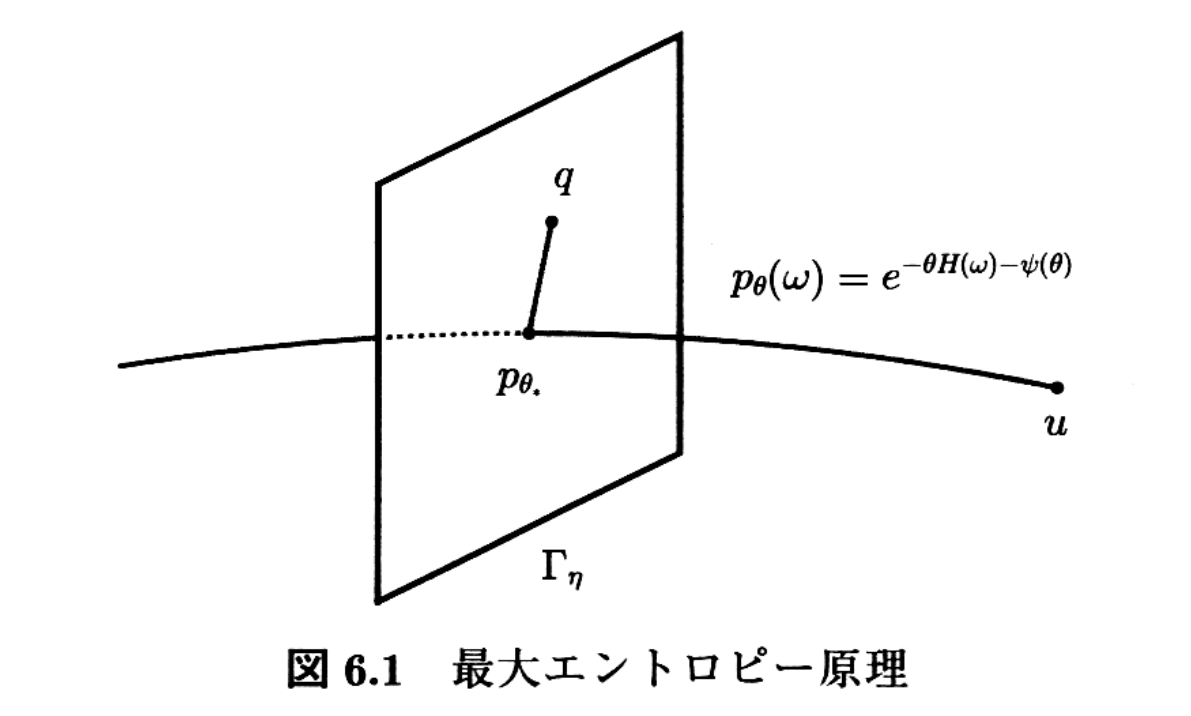
\includegraphics[width=100mm]{entropy.png}
    \end{center}
    \caption{エネルギー期待値が一定の面の中で一様分布に最も近い分布が$p_{\theta_*}$である。}
    \label{fig:one}
\end{figure}

ところで、
\begin{align}
    \log Z(\theta) &= \Psi(\theta)\\
    \beta &= \theta_{*}
\end{align}
とおくと、
\begin{align}
    \underset{\ev{H} = \text{const}}{\text{argmax}} \{S(q)\} &= p_{\beta}(\omega)\\
    &= \exp\left[ -\beta H(\omega) - \psi(\beta) \right]\\
    &= \frac{1}{Z(\beta)} \exp\left[ -\beta H(\omega) \right]
\end{align}
となり、見慣れたカノニカル分布の形になる。\\
以上をまとめると、最大エントロピー原理は、情報幾何の立場では、拘束条件のもとで、一様分布分布との距離のようなもの(KLダイバージェンス)を最小しようという話になる。\\

また、測地線の式の両辺の対数をとって、$p_{\theta}$に関する期待値をとると、
\begin{align}
    \Psi(\theta) &= S(p_{\theta}) - \theta E_{p_{\theta}}[H]
\end{align}
となる。このとき、$\mathcal{S}$の任意の確率分布$r$と、カノニカル分布$p_{\beta}$とのKLダイバージェンスは、
\begin{align}
    D(r||p_{\beta}) &= \sum_{\omega \in \Omega} r(\omega) \log \frac{r(\omega)}{p_{\beta}(\omega)}\\
    &= -S(r) \beta E_r[H] + \Psi(\beta)\\
    &= -(S(r) - \beta E_r[H]) + (S(p_{\beta}) - \beta E_{p_{\beta}}[H])
\end{align}
となる。したがって、ダイバージェンスの正値性から、
\begin{align}
    S(p_{\beta}) - \beta E_{p_{\beta}}[H] \geq S(r) - \beta E_r[H]
\end{align}
となる。ここで、
\begin{align}
    F(r) = E_r[H] - \frac{1}{\beta}S(r)
\end{align}
とおくと、
\begin{align}
    p_{\beta} = \underset{r}{\text{argmin}} F(r)
\end{align}
となる。これは、自由エネルギーの最小化原理である。注意されたいこととして、自由エネルギーを最小化するという立場では、拘束条件は特にない。\\
こうして、拘束条件の下での最小化問題を、拘束条件なしでの最小化問題に言い換えられたわけだが、この議論で鍵になったのはKLダイバージェンスの正値性であった。ところで、ダイバージェンスの正値性はルジャンドル変換と結びついていた。したがって、エントロピーと自由エネルギーとの関係がルジャンドル変換によって表されるのではないかと考えられる。\footnote{物理の人はルジャンドル変換を最初から用いることが多い。}\\
今、ダイバージェンスの正値性と同等なルジャンドル変換の関係式は、
\begin{align}
    \psi(\theta_\beta) = \max_{r \in \mathcal{S}}\{\theta^i(p_\beta)\eta_i(r) - \varphi(\eta(r))\}
\end{align}
であった。いま、
\begin{align}
    \theta^1(p_\beta) &= \beta\\
    \theta^n(p_\beta) &= 0 \quad (n\geq 2)\\
    \eta_1(r) &= -E_r[H]\\
    \phi(\eta(r)) &= -S(r)
\end{align}
であるから、
\begin{align}
    \log Z(\theta(p_\beta)) = \max_{r \in \mathcal{S}}\{-\beta E_r[H] + S(r)\}
\end{align}
となる。とくに$\beta >0$のとき、
\begin{align}
    -\frac{1}{\beta}\log Z(\theta(p_\beta)) = \min_{r \in \mathcal{S}}\{E_r[H] - \frac{1}{\beta}S(r)\}
\end{align}
となる。この右辺は自由エネルギーであり、とくに$r = p_\beta$のとき最小値をとる。したがって、
\begin{align}
    -\frac{1}{\beta}\log Z(\theta(p_\beta)) = F(p_\beta)
\end{align}
となる。これは統計物理においてよく知られた関係式である。\\

\end{document}